\chapter{Analyse verschiedener Fahrszenarien und Interpretation des Lösungsraumes}\label{cha:Ergebnisse}
In diesem Kapitel wird das im vorangegangenen Kapitel hergeleitete Gesamtsystem mit den Methoden aus Kapitel \ref{cha:Optimierung} für verschiedene Fahrszenarien gelöst. Dazu werden zunächst einige Vereinfachungen getroffen, mit denen es teilweise möglich ist, eine analytische Lösung zu finden. Die Erkenntnisse der einfacheren Szenarien werden dann verwendet, um die Lösungen komplexerer Szenarien zu interpretieren. 

\section{Geradeausfahrt}\label{sec:Geradeausfahrt}
Als erstes wird das Szenario einer reinen Geradeausfahrt betrachtet. Dazu wird das Fahrzeugmodell auf die Bewegung in longitudinaler Richtung reduziert und angenommen, dass sich das Fahrzeug exakt auf der Referenzkurve mit $\kapparefofs = 0$ bewegt -- die querdynamischen Größen $d_r, \psi_r$ und $\kappa$ werden dabei vernachlässigt. Da sich das Fahrzeug auf der Referenzkurve befindet, ist durch $s_r$ die exakt vom Fahrzeug zurückgelegte Strecke gegeben. Die Systemdynamik des Fahrzeugs ist dann durch die Gleichungen 
\begin{align}
\dot{s}_r &= v \\
\dot{v} &= a_x \\
\dot{a}_x &= j_x \,,
\end{align}
vollständig beschrieben -- es ergibt sich ein Integratorsystem 3. Ordnung. Die einzige Stellgröße ist in diesem Fall der Längsruck $j_x$.

\subsection{Lösungsraum bei energieoptimalem Gütefunktional}\label{subsec:Lösungsraum_Geradeausfahrt}
Zunächst wird die Lösung des Szenarios Geradeausfahrt für ein energieoptimales Gütefunktional bestimmt. Wird im Gütefunktional die Stellgröße eines Systems bestraft, so wird von einem energieoptimalen Gütefunktional gesprochen, da das Ziel der Optimierung darin besteht, die benötigte Stellgröße möglichst gering zu halten. Diese ist häufig direkt mit der aufzuwendenden Energie verknüpft \cite{KnutGraichen.2012}. Wird zusätzlich noch die Endzeit als Gütekriterium bestraft, so ergibt sich in dem vereinfachten Szenario Geradeausfahrt das Gütefunktional
\begin{equation}
	J(\ve{x},\ve{u},t,t_f) = t_f + \int_{t_0}^{t_f}\frac{1}{2}f_uu^2~\dtint{t} = t_f + \int_{t_0}^{t_f}\frac{1}{2}\fjx j_x^2~\dtint{t}\,.
\end{equation}
Die Formulierung eines Integratorsystems mit einem energieoptimalen Gütefunktional soll nachfolgend verallgemeinert betrachtet werden. Wird die Stellgröße eines Integratorsystems mit der Ordnung $n$ als die $n$-te Ableitung des ersten Zustands gewählt, kann das Gütefunktional als 
\begin{equation}
J(\ve{x},\ve{u},t,t_f) = t_f + \int_{t_0}^{t_f}\frac{1}{2}f_u{x_1^{(n)}}^2~\dtint{t}\,.
\end{equation}
geschrieben werden, wobei der eingeklammerte Hochindex $(n)$ die $n$-te Zeitableitung bezeichnet. Die Hamilton-Funktion ergibt sich zu
\begin{equation}
H(\ve{x},\ve{u},\ve{\lambda},t) = \frac{1}{2}f_u{x_1^{(n)}}^2 + \lambda_1x_1^{(1)} + \lambda_2x_1^{(2)} + ... + \lambda_nx_1^{(n)}
\end{equation}
und die adjungierten \gls{DGL} lauten dann  
\begin{align}
	\dot{\lambda_1} &= 0 \\
	\dot{\lambda_2} &= -\lambda_1 \\
	&\vdots \\
	\dot{\lambda_n} &= -\lambda_{n-1}\,.
\end{align}
Daraus wird ersichtlich, dass sich mit $x_1^{(n)} = -\frac{\lambda_n}{f_u}$ alle Zeitverläufe durch Integration ausgehend von $\lambda_1 = \textrm{konst.}$ bestimmen lassen. Dabei erhält man Polynome deren Grad mit jeder Integration um eins steigt. Bei einem System $n$-ter Ordnung müssen insgesamt $2n$ Integrationen durchgeführt werden, sodass die Lösung von $x_1$ ein Polynom vom Grad $2n-1$ darstellt. Der höchste Polynomgrad ist also immer ungerade. Dabei lässt sich feststellen, dass der Einfluss der höheren Exponenten der Polynome durch die mehrfache Integration abnimmt. Der Lösungsraum lässt sich wie folgt geschlossen angeben: 
\begin{align}
\begin{split}
\lambda_1 &= c_1 
\end{split}
\\
\begin{split}
\lambda_2 &= -c_1t + c_2 
\end{split}
\\
\begin{split}
&\vdots 
\end{split}
\\
\begin{split}
\lambda_n &= (-1)^{n-1}\frac{c_1}{(n-1)!}t^{n-1} + (-1)^{n-2}\frac{c_2}{(n-2)!}t^{n-2} + ... + (-1)^1c_{n-1}t + c_n 
\end{split}
\\
\begin{split}
x_n &= (-1)^n\frac{c_1}{f_u(n)!}t^{n} + (-1)^{n-1}\frac{c_2}{(n-1)!}t^{n-1} + ... - \frac{c_{n}}{f_u}t + x_{n,0} 
\end{split}
\\
\begin{split}
x_{n-1} &= (-1)^n\frac{c_1}{f_u(n+1)!}t^{n+1} + (-1)^{n-1}\frac{c_2}{(n)!}t^{n} + ... - \frac{c_{n}}{2f_u}t^2 + x_{n,0}t + x_{n-1,0} 
\end{split}
\\
\begin{split}
&\vdots 
\end{split}
\\
\begin{split}
x_{1} &= (-1)^n\frac{c_1}{f_u(2n-1)!}t^{2n-1} + (-1)^{n-1}\frac{c_2}{(2n-2)!}t^{2n-2} + ... - \frac{c_{n}}{f_u(n)!}t^n + ... \\
&\qquad ... + \frac{x_{n,0}}{(n-1)!}t^{n-1} + \frac{x_{n-1,0}}{(n-2)!}t^{n-2} + ... + x_{2,0}t + x_{1,0}
\end{split}
\end{align}
Damit lautet die Lösung des Integratorsystems 3. Ordnung für die Geradeausfahrt
\begin{align}
\begin{split}
\lambda_1 &= c_1 
\end{split}
\\
\begin{split}
\lambda_2 &= -c_1t + c_2 
\end{split}
\\
\begin{split}
\lambda_3 &= \frac{c_1}{2}t^2 - c_2t + c_3 
\end{split}
\\
\begin{split}
a_x &= -\frac{c_1}{6\fjx}t^3 + \frac{c_2}{2\fjx}t^2 - \frac{c_3}{\fjx}t + c_a
\end{split}
\\
\begin{split}
v &= -\frac{c_1}{24\fjx}t^4 + \frac{c_2}{6\fjx}t^3 - \frac{c_3}{2\fjx}t^2 + c_at + c_v
\end{split}
\\
\begin{split}
s &= -\frac{c_1}{120\fjx}t^5 + \frac{c_2}{24\fjx}t^4 - \frac{c_3}{6\fjx}t^3 + \frac{c_a}{2}t + c_vt + c_s
\end{split}
\end{align}
Letztendlich können die in den Gleichungen auftretenden unbekannten Integrationskonstanten $c_1, c_2, c_3,$ $c_a, c_v$ und $c_s$ mithilfe der Randbedingungen \eqref{eq:Anfangswerte}--\eqref{eq:Lambdaend} bestimmt und damit das \gls{OP} gelöst werden. Im Fall, dass der Endzeitpunkt frei ist, kann $t_f$ unter Zuhilfenahme von Gleichung \eqref{eq:Transversalitaet} bestimmt werden. Die dynamischen Gleichungen des Gesamtsystems können auch in der für die Beschreibung linearer Systeme üblichen Matrixschreibweise $\dz = \mat{A}\ve{z}$ geschrieben werden. Mit $\ve{z} = \begin{bmatrix}\ve{x}^T & \ve{\lambda}^T\end{bmatrix}^T$ lautet das lineare System \begin{equation}
	\dz = \begin{bmatrix}
	0 & 1 & 0 & 0 & 0 & 0 \\
	0 & 0 & 1 & 0 & 0 & 0 \\
	0 & 0 & 0 & 0 & 0 & -\frac{1}{\fjx} \\
	0 & 0 & 0 & 0 & 0 & 0 \\
	0 & 0 & 0 & -1 & 0 & 0 \\
	0 & 0 & 0 & 0 & -1 & 0 \\
	\end{bmatrix}\ve{z}\,,
\end{equation}
dessen Eigenwerte erwartungsgemäß alle in Null liegen und das reine Integrationsverhalten des Systems widerspiegeln.

\subsection{Lösungsraum bei Gütefunktional mit Bestrafung von Längsruck und -beschleunigung}\label{subsec:Lösungsraum_ax_jx}
Wird nun neben dem energieoptimalen Anteil noch die ebenfalls komfortrelevante Größe Längsbeschleunigung berücksichtigt, lautet das Gütefunktional für die Geradeausfahrt 
\begin{equation}
J(\ve{x},\ve{u},t,t_f) = t_f + \int_{t_0}^{t_f}\frac{1}{2}\fjx j_x^2 + \frac{1}{2}\fax a_x^2~\dtint{t}\,.
\end{equation}
Analog zum Vorgehen aus dem vorherigen Abschnitt können die adjungierten \gls{DGL} aufgestellt werden. Diese lauten nun
\begin{align}
\dot{\lambda_1} &= 0 \\
\dot{\lambda_2} &= -\lambda_1 \\
\dot{\lambda_3} &= -(\fax a_x + \lambda_2)\,. \label{eq:dlambda3_Geradeausfahrt}
\end{align}
Das lineare System lässt sich mit \begin{equation}
\dz = \begin{bmatrix}
0 & 1 & 0 & 0 & 0 & 0 \\
0 & 0 & 1 & 0 & 0 & 0 \\
0 & 0 & 0 & 0 & 0 & -\frac{1}{\fjx} \\
0 & 0 & 0 & 0 & 0 & 0 \\
0 & 0 & 0 & -1 & 0 & 0 \\
0 & 0 & -\fax & 0 & -1 & 0 \\
\end{bmatrix}\ve{z}
\end{equation}
angeben und besitzt im Gegensatz zu dem linearen System aus dem vorherigen Abschnitt zwei Eigenwerte bei $\pm\sqrt{\frac{\fax}{\fjx}}$. Die restlichen vier Eigenwerte liegen auch bei diesem System in Null. Es zeigt sich allerdings, dass neben dem integrierenden Verhalten auch stabile und instabile Eigenmoden auftreten. Auch in diesem Fall lässt sich die Lösung der \gls{DGL} analytisch berechnen. Die Lösung von $\lambda_2$ kann durch Integration der Konstanten $c_1$ bestimmt werden. Wird die Steuerungsgleichung $j_x = -\frac{\lambda_3}{\fjx}$ abgeleitet und in Gleichung \eqref{eq:dlambda3_Geradeausfahrt} eingesetzt, ergibt sich für die Beschleunigung eine gewöhnliche \gls{DGL} 2. Ordnung. Durch das Einsetzen erhält man die \gls{DGL}
\begin{equation}
\dot{j}_x = \ddot{a}_x = \frac{\fax}{\fjx}a_x + \frac{\lambda_2}{\fjx} = \frac{\fax}{\fjx}a_x - \frac{c_1}{\fjx}t + \frac{c_2}{\fjx} \,, \label{eq:DGL_ax}
\end{equation}
deren Lösung
\begin{equation}
a_x = k_1e^{\sqrt{\frac{\fax}{\fjx}}t} + k_2e^{-\sqrt{\frac{\fax}{\fjx}}t} + \frac{c_1}{\fax}t - \frac{c_2}{\fax} \, \label{eq:DGL_ax_Lösung}
\end{equation}
lautet, wobei die Faktoren $k_1$ und $k_2$ Konstanten bezeichnen, die bei der Lösung der \gls{DGL} entstehen. Durch zeitliches Differenzieren bzw. Integrieren können aus $a_x$ die Lösungen für $j_x, v$ und $s_r$ ermittelt werden. Diese lauten
\begin{align}
\begin{split}
j_x &= k_1\sqrt{\frac{\fax}{\fjx}}e^{\sqrt{\frac{\fax}{\fjx}}t} - k_2\sqrt{\frac{\fax}{\fjx}}e^{-\sqrt{\frac{\fax}{\fjx}}t} + \frac{c_1}{\fax} \label{eq:DGL_jx_Lösung}
\end{split}
\\
\begin{split}
v &= k_1\sqrt{\frac{\fjx}{\fax}}e^{\sqrt{\frac{\fax}{\fjx}}t} - k_2\sqrt{\frac{\fjx}{\fax}}e^{-\sqrt{\frac{\fax}{\fjx}}t} + \frac{c_1}{2\fax}t^2 - \frac{c_2}{\fax}t + c_v
\end{split}
\\
\begin{split}
s &= k_1\frac{\fjx}{\fax}e^{\sqrt{\frac{\fax}{\fjx}}t} + k_2\frac{\fjx}{\fax}e^{-\sqrt{\frac{\fax}{\fjx}}t} + \frac{c_1}{6\fax}t^3 - \frac{c_2}{2\fax}t^2 + c_vt + c_s \,.
\end{split}
\end{align}
Auch hier bestehen die Lösungen der Trajektorien zum Teil aus Polynomen. Allerdings sind die Polynomgrade um zwei geringer als bei der reinen energieoptimalen Lösung. Des Weiteren zeigt sich mit den Exponentialtermen der Einfluss der stabilen und instabilen Moden auf die Systemzustände. Es kann festgestellt werden, dass die optimalen Trajektorien mit geringerer Bestrafung der Längsbeschleunigung zunehmend gegen die Lösung der rein ruckoptimalen Lösung laufen, wie in Abbildung \ref{fig:var_fax} zu erkennen ist. Offenbar ergeben sich die Koeffizienten $k_1$ und $k_2$ der Exponentialanteile bei der Lösung des nichtlinearen Gleichungssystems derart, dass der Einfluss der \glqq fehlenden\grqq~Polynomgrade durch die Exponentialfunktionen ersetzt wird. Die Abbildung macht außerdem deutlich, dass bereits eine Bestrafung der Längsbeschleunigung von $\fax = 0.05$, die um den Faktor 20 geringer ist, als die Bestrafung des Längsrucks, zu wesentlich niedrigeren Beschleunigungsverläufen und damit einem höheren Maß an Fahrkomfort führt. Dies geschieht auf Kosten der Reisezeit, da diese entsprechend ansteigt. 
\begin{figure}[h] 
	\centering
	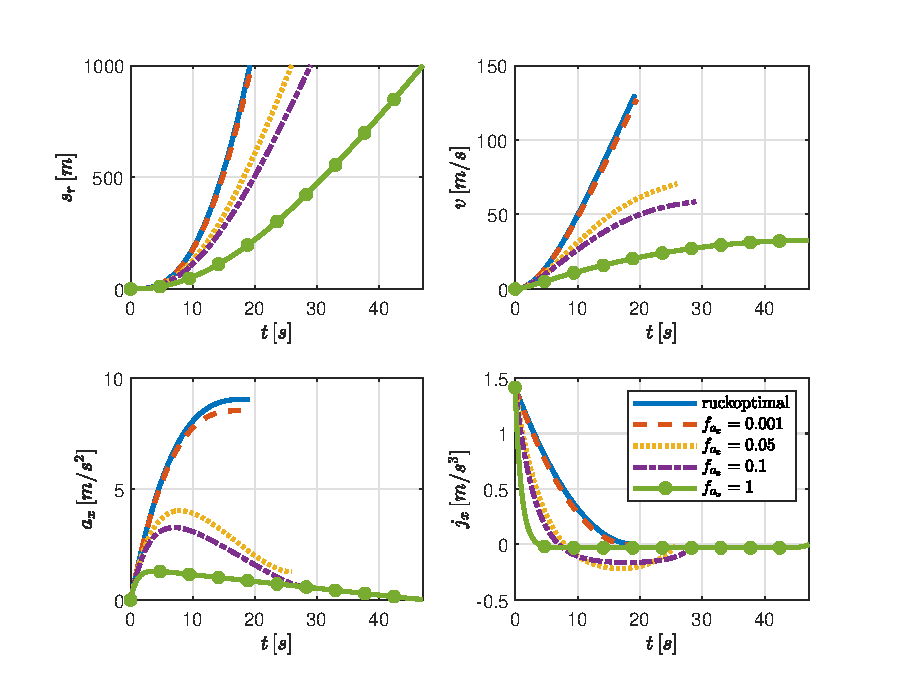
\includegraphics[width=0.8\linewidth]{./Bilder/Ergebnisse/Geradeausfahrt/var_fax.eps}
	\caption{Lösungstrajektorien der Fahrzeugzustände und der Stellgröße bei einer Geradeausfahrt mit $s_f=\valunit{1000}{m}$ und freien Endzuständen und freier Endzeit. Für abnehmende Bestrafung der Längsbeschleunigung nimmt die optimale Lösung immer mehr die Form der rein ruckoptimalen Lösung an. Der Ruck ist dabei mit $\fjx = 1$ gewichtet.}
	\label{fig:var_fax}
\end{figure}

\subsection{Lange Geradeausfahrt}
Ein Szenario, in dem die bisherigen Ergebnisse Anwendung finden ist die lange Geradeausfahrt, die nachfolgend eingehend analysiert werden soll. Zunächst wird die Lösung für die Standardparametrierung der Gewichtungsfaktoren, also für gleiche Bestrafung von Beschleunigung und Ruck betrachtet. Das Szenario einer langen Geradeausfahrt zeichnet sich dadurch aus, dass sich der Zeitverlauf in drei Abschnitte unterteilen lässt. Im ersten Bereich für kleine Zeitpunkte gilt $0\leq t\ll t_f$, während im dritten Bereich nahe des Endzeitpunkts $0\ll t\leq t_f$ gilt. In dem Bereich dazwischen gilt $0\ll t\ll t_f$. Es zeigt sich, dass der Koeffizient des instabilen Teils $k_1$ sehr geringe Werte im Bereich von $10^{-40}\leq k_1 \leq 10^{-10}$ annimmt, wobei $k_2$ um einige Größenordnungen größer ist. Dies hat zur Folge, dass der Einfluss des instabilen Anteils erst für große $t$ (im dritten Zeitabschnitt) sichtbar wird und die Trajektorien divergieren, während das Verhalten für kleine $t$ (im ersten Zeitabschnitt) vom stabilen Teil dominiert wird und anschließend abklingt. Im Bereich dazwischen ist der Einfluss des stabilen Anteils bereits abgeklungen und der instabile Anteil ist noch nicht aufgeklungen. Folglich lässt sich die Aussage treffen, dass die Trajektorien für $t\ll t_f$ von links und für $0\ll t$ von rechts gegen den Polynomanteil konvergieren. Unter der Voraussetzung, dass die beiden Exponentialanteile jeweils nur in einem der drei Bereiche gelten, lassen sich die folgenden Annahmen treffen. Für den ersten Bereich kann der Einfluss der instabilen Mode mit $k_1(\cdot)e^{\sqrt{\frac{\fax}{\fjx}}t} \approx 0$ angenommen werden. Analog dazu gilt für den Einfluss des stabilen Anteils im dritten Bereich $k_2(\cdot)e^{-\sqrt{\frac{\fax}{\fjx}}t} \approx 0$. In diesen Bereichen gilt 
\begin{align}
j_x &\approx -k_2\sqrt{\frac{\fax}{\fjx}}e^{-\sqrt{\frac{\fax}{\fjx}}t} + \frac{c_1}{\fax} \quad\textrm{für}\quad 0\leq t\ll t_f \label{eq:j_Bereich_1} \\
a_x &\approx k_2e^{-\sqrt{\frac{\fax}{\fjx}}t} + \frac{c_1}{\fax}t - \frac{c_2}{\fax} \quad\textrm{für}\quad 0\leq t\ll t_f\,. \label{eq:a_Bereich_1}
\end{align}
sowie 
\begin{align}
j_x &\approx k_1\sqrt{\frac{\fax}{\fjx}}e^{\sqrt{\frac{\fax}{\fjx}}t} + \frac{c_1}{\fax} \quad\textrm{für}\quad 0\ll t\leq t_f \label{eq:j_Bereich_3} \\
a_x &\approx k_1e^{\sqrt{\frac{\fax}{\fjx}}t} + \frac{c_1}{\fax}t - \frac{c_2}{\fax} \quad\textrm{für}\quad 0\ll t\leq t_f\,. \label{eq:a_Bereich_3}
\end{align}
Die Trajektorien im zweiten Bereich lassen sich durch ihre Polynomanteile approximieren. Für die komfortrelevanten Größen Ruck und Beschleunigung gilt dann
\begin{align}
j_x &\approx \frac{c_1}{\fax} \quad\textrm{für}\quad 0\ll t\ll t_f \label{eq:j_Bereich_2}
\\
a_x &\approx \frac{c_1}{\fax}t - \frac{c_2}{\fax} \quad\textrm{für}\quad 0\ll t\ll t_f\,. \label{eq:a_Bereich_2}
\end{align}
Da die Trajektorien des Rucks und der Beschleunigung für lange Geradeausfahrten offenbar als Konstante bzw. Gerade betrachtet werden können, zu denen die Lösung sowohl von links als auch von rechts hin konvergiert, stellt sich die Frage, ob anhand der Kenntnis über den Lösungsraum, Beschränkungen für die Längsbeschleunigung angegeben werden können. 

\subsubsection{Begrenzung der Längsbeschleunigung}\label{subsubsec:Begrenzung_ax}
Nachfolgend werden zwei Sets von Randbedingungen untersucht. Kenntnis über die Anfangszustände und damit Vorgabe der Anfangsbedingungen \xzero~wird bei allen Szenarien vorausgesetzt. Allerdings kann die Vorgabe der Endwerte variiert werden. Zwei Sets an Endbedingungen erweisen sich bei der hier betrachteten langen Geradeausfahrt als besonders geeignet. Neben der Vorgabe einer Strecke $s_f$, die zurückgelegt werden soll und damit der Vorgabe des Endzustands für $s_r(t_f)$, können die Endgeschwindigkeit und -beschleunigung entweder festgelegt oder frei sein. Die Vorgabe von Endgeschwindigkeit und -beschleunigung ist sinnvoll, wenn das Fahrzeug unter Berücksichtigung des Gütefunktionals beispielsweise nach einer festgelegten Strecke unbeschleunigt zum Stehen gebracht werden soll. Wenn hingegen diese beiden Endzustände nicht festgelegt sind, weil das Ziel nur darin besteht, die vorgegebene Strecke unter Berücksichtigung des Gütefunktionals abzufahren, dann können diese Endzustände frei bleiben, wobei sich nach Gleichung \eqref{eq:Lambdaend} Endbedingungen für die adjungierten Zustände ergeben. 

\textbf{Feste Endgeschwindigkeit und feste Endbeschleunigung}

Zur Klärung der Frage, ob die Längsbeschleunigung beschränkt ist, kann eine Fallunterscheidung für die Vorzeichen der Koeffizienten $k_1$ und $k_2$ vorgenommen werden. So lässt sich feststellen, dass der stabile und instabile Anteil in Gleichung \eqref{eq:DGL_ax_Lösung} bei identischem Vorzeichen die gleiche Krümmungsrichtung haben (unabhängig davon, ob das Vorzeichen positiv oder negativ ist). Das bedeutet, dass die Exponentialanteile entweder beide von oben oder beide von unten gegen den linearen Lösungsanteil konvergieren. Für den Ruck bedeuten identische Vorzeichen, dass die Krümmungen der Exponentialanteile in der Lösung in Gleichung \eqref{eq:DGL_jx_Lösung} immer entgegengesetzte Richtungen haben und einer der Anteile von oben gegen die Konstante konvergiert, während der andere Teil von unten gegen die Konstante läuft. Aufgrund des streng monotonen Verhaltens der Exponentialfunktionen, ist auch der Ruck über das gesamte Lösungsintervall streng monoton, sodass $j_x$ genau eine Nullstelle hat. Dadurch, dass der Ruck genau eine Nullstelle besitzt, hat $a_x$ genau ein Extremum. Mit der Kenntnis, dass die Beschleunigung ausgehend vom Anfangswert $a_0$ gegen die Gerade in Bereich zwei konvergiert und anschließend unter Beibehaltung der Krümmungrichtung von der Geraden weg gegen den Endwert $a_f$ läuft, lasst sich feststellen, dass die Beschleunigung bei gleichem Vorzeichen der Koeffizienten $k_1$ und $k_2$ stets durch den linearen Anteil der Lösung und die Verbindungsgerade zwischen $a_0$ und $a_f$ beschränkt ist. In Abbildung \ref{fig:vf_af_fest_gleiches_VZ} sind die optimalen Lösungstrajektorien der Fahrzeugzustände $s_r$, $v$ und $a_x$ sowie der Stellgröße $j_x$ bei vorgegebenen Endzuständen und ansonsten identischer Parametrierung dargestellt. 
\begin{figure}[h] 
	\centering
	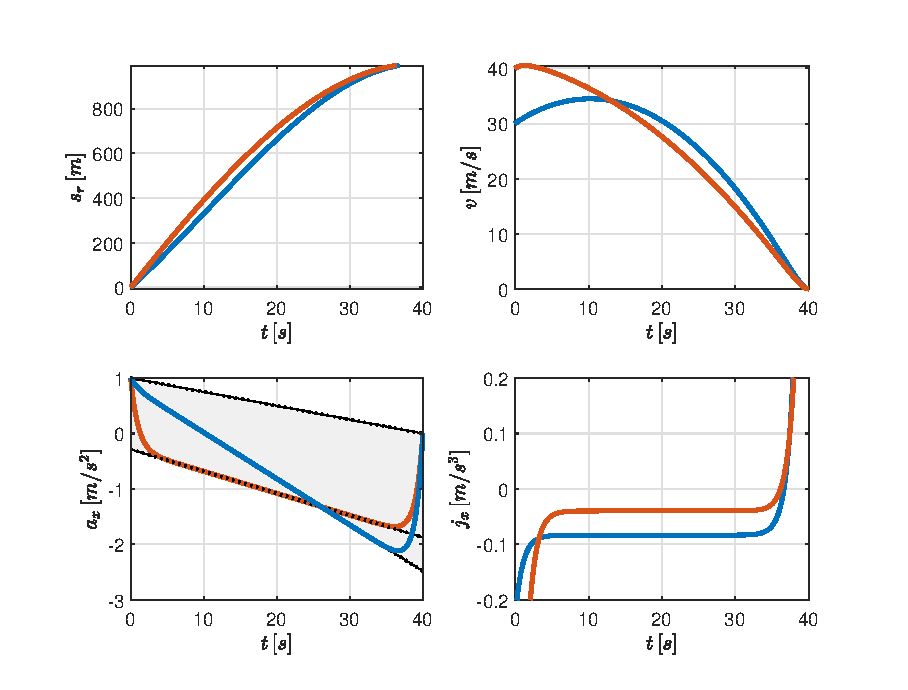
\includegraphics[width=\linewidth]{./Bilder/Ergebnisse/Geradeausfahrt/vf_af_fest_gleiches_VZ.eps}
	\caption{Lösungstrajektorien der Fahrzeugzustände und der Stellgröße bei einer langen Geradeausfahrt mit $s_f=\valunit{1000}{m}$ und fester Endgeschwindigkeit und -beschleunigung. Das Vorzeichen von $k_1$ und $k_2$ ist identisch. Der Endzeitpunkt beträgt $t_f = \valunit{40}{s}$.}
	\label{fig:vf_af_fest_gleiches_VZ}
\end{figure}
Die Anfangsgeschwindigkeit wird so gewählt, dass die Vorzeichen der Lösungen von $k_1$ und $k_2$ identisch sind. Die Endzustände werden so gewählt, dass das Fahrzeug nach \valunit{1000}{m} unbeschleunigt zum Stehen kommt. Der Endzeitpunkt wird im Sinne einer einheitlichen Darstellung fest zu $t_f = \valunit{40}{s}$ gewählt. Das zuvor beschriebene Verhalten der Beschleunigungs- und Rucktrajektorien ist gut in den unteren beiden Graphen zu erkennen. Zum einen lassen sich die beiden Bereiche erkennen, in denen die Lösungen von den Exponentialteilen dominiert werden, sowie der mittlere Bereiche, in dem die Lösungen der Geraden für die Beschleunigung und der Konstanten für den Ruck entsprechen. Zudem zeigt die Abbildung unten links die Beschränkung der Beschleunigung (grau schattiert) durch die Verbindungsgerade der Randwerte und den linearen Anteil der Lösung.

Für den Fall, dass das Vorzeichen der Koeffizenten $k_1$ und $k_2$ unterschiedlich ist, haben die Exponentialanteile in $j_x$ dieselbe Krümmungsrichtung und laufen damit beide entweder von oben oder von unten gegen die Konstante, während die Anteile in $a_x$ mit unterschiedlichen Vorzeichen wirken. Damit lässt sich feststellen, dass $j_x$ immer zwei Nullstellen besitzt, weshalb in $a_x$ zwei Extrema auftreten können. Da $j_x$ bei zwei Nullstellen einen Vorzeichenwechsel aufweist, hat die Steigung der Beschleunigung einen Richtungswechsel, woraus abgeleitet werden kann, dass es bei zwei Extrema ein Maximum und ein Minimum gibt und die Lösung von $a_x$ die Verbindungsgerade der Randwerte in einem Punkt schneidet. Dadurch, dass die Exponentialanteile der Lösung auch hier wieder gegen den linearen Anteil konvergieren, kann schließlich auch in diesem Fall argumentiert werden, dass die Beschleunigung stets durch die Verbindungsgerade von $a_0$ und $a_f$ und den linearen Anteil beschränkt ist, wobei sich die Geraden im mittleren Abschnitt bei 
\begin{equation}
t = \frac{a_0\fax + c_2}{c_1 - \frac{\fax(a_f - a_0)}{t_f}}
\end{equation} 
schneiden. Das Verhalten für diesen Lösungsfall ist in Abbildung \ref{fig:vf_af_fest_unterschiedliches_VZ} dargestellt. In den Graphen der Beschleunigung und des Rucks zeigt sich deutlich das beschriebene Verhalten mit den unterschiedlich gekrümmten Exponentialanteilen sowie die Konvergenz von links und rechts hin zu der jeweiligen Lösung auf dem mittleren Abschnitt. Außerdem ist die Beschränkung der Beschleunigung gut zu erkennen. 
\begin{figure}[h] 
	\centering
	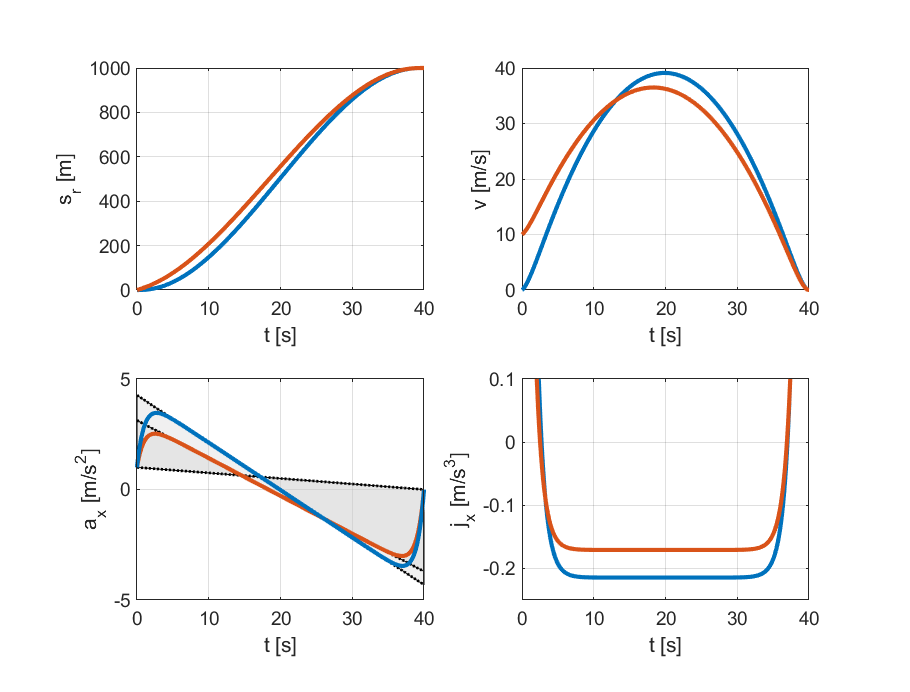
\includegraphics[width=\linewidth]{./Bilder/Ergebnisse/Geradeausfahrt/vf_af_fest_unterschiedliches_VZ.eps}
	\caption{Lösungstrajektorien der Fahrzeugzustände und der Stellgröße bei einer langen Geradeausfahrt mit $s_f=\valunit{1000}{m}$ und fester Endgeschwindigkeit und -beschleunigung. Das Vorzeichen von $k_1$ und $k_2$ ist unterschiedlich. Der Endzeitpunkt beträgt $t_f = \valunit{40}{s}$.}
	\label{fig:vf_af_fest_unterschiedliches_VZ}
\end{figure}

\textbf{Freie Endgeschwindigkeit und freie Endbeschleunigung}

Dadurch, dass die Endzustände $v(t_f)$ und $a_x(t_f)$ nicht festgelegt sind, ergeben sich die Endbedingungen $\lambda_2(t_f) = 0$ und $\lambda_3(t_f) = 0 \rightarrow j_x(t_f) = 0$. Bei dieser Wahl der Endbedingungen ist die analytische Herleitung der maximalen und minimalen Beschleunigung möglich, welche nachfolgend betrachtet werden soll. Da $j_x$ bis auf die beiden Exponentialanteile konstant ist, kann argumentiert werden, dass der Ruck maximal zwei Nullstellen aufweist, wobei diese nicht in Bereich zwei liegen können (in diesem Bereich ist $j_x$ näherungsweise konstant). Ein Kontinuum an Nullstellen in Bereich zwei ist aufgrund des monotonen Verhaltens der Exponentialfunktionen nicht möglich, weshalb der Ruck im ersten und im dritten Bereich auf Nullstellen untersucht wird. Im ersten Bereich folgt mit $j_x \stackrel{!}{=} 0$ aus Gleichung \eqref{eq:j_Bereich_1}
\begin{equation}
	t_{z,1} = -\sqrt{\frac{\fjx}{\fax}}\ln{\Big(\frac{c_1}{k_2}\sqrt{\frac{\fjx}{\fax^3}}\Big)}\,. \label{eq:t_z_1}
\end{equation}
Dadurch, dass die Endgeschwindigkeit frei ist, ergibt sich die Endbedingung 
\begin{equation}
	\lambda_2(t_f) = -c_1t_f + c_2 \stackrel{!}{=} 0\,.
\end{equation}
Mit der Anfangsbedingung für die Beschleunigung $a_x(0) = a_0$ folgt aus Gleichung \eqref{eq:a_Bereich_1}
\begin{equation}
k_2 = a_0 + \frac{c_2}{\fax} = a_0 + \frac{c_1t_f}{\fax}\,.
\end{equation}
Wird dieser Zusammenhang in Gleichung \eqref{eq:t_z_1} eingesetzt, erhält man mit 
\begin{equation}
t_{z,1} = -\sqrt{\frac{\fjx}{\fax}}\ln{\Big(\frac{c_1}{a_0+\frac{c_1t_f}{\fax}}\sqrt{\frac{\fjx}{\fax^3}}\Big)}
\end{equation}
den Zeitpunkt des Nulldurchgang von $j_x$ im ersten Bereich, wobei dieser vom Anfangswert der Beschleunigung, den Gewichtungsfaktoren der Komfortkriterien, dem Endzeitpunkt und der Lösung von $\lambda_1$ abhängt. Einsetzen von $t_{z,1}$ in Gleichung \eqref{eq:a_Bereich_1} liefert den Extremwert der Beschleunigung an dieser Stelle mit 
\begin{equation}
a_{x_{z,1}} = c_1\sqrt{\frac{\fjx}{\fax^3}} -c_1\sqrt{\frac{\fjx}{\fax^3}}\ln{\Big(\frac{c_1}{a_0+\frac{c_1t_f}{\fax}}\sqrt{\frac{\fjx}{\fax^3}}\Big)} - \frac{c_1t_f}{\fax}\,. 
\end{equation}
Die zweite Nullstelle von $j_x$ resultiert in dieser Wahl der Randbedingungen direkt aus $j_x(t_f) = 0$. Der Ruck hat folglich immer bei $t_{z,2} = t_f$ ein Extremum. Aus Gleichung \eqref{eq:j_Bereich_3} folgt 
\begin{equation}
k_1 = -\frac{c_1\sqrt{\frac{\fjx}{\fax^3}}}{e^{\sqrt{\frac{\fax}{\fjx}}t_f}}\,.
\end{equation}
Eingesetzt in Gleichung \eqref{eq:a_Bereich_3} lautet die Beschleunigung der zweiten Extremstelle
\begin{equation}
a_{x_{z,2}} = -c_1\sqrt{\frac{\fjx}{\fax^3}} + \frac{c_1}{\fax}t_f - \frac{c_1t_f}{\fax} = -c_1\sqrt{\frac{\fjx}{\fax^3}}\,. 
\end{equation}
Es lässt sich also festhalten, dass bei freien Endzuständen eine Extremstelle der Beschleunigung bei $t_f$ liegt und eine im ersten Abschnitt. Da der Endwert der Beschleunigung bei positiver Steigung immer unter dem linearen Lösungsanteil und bei negativer Steigung oberhalb der Geraden liegt, ist die Beschränkung durch den linearen Anteil der Lösung streng genommen nicht mehr gültig. Dennoch ist die Gerade als Näherungslösung für die Beschränkung geeignet wie Abbildung \ref{fig:vf_af_frei} zeigt. 
\begin{figure}[h] 
	\centering
	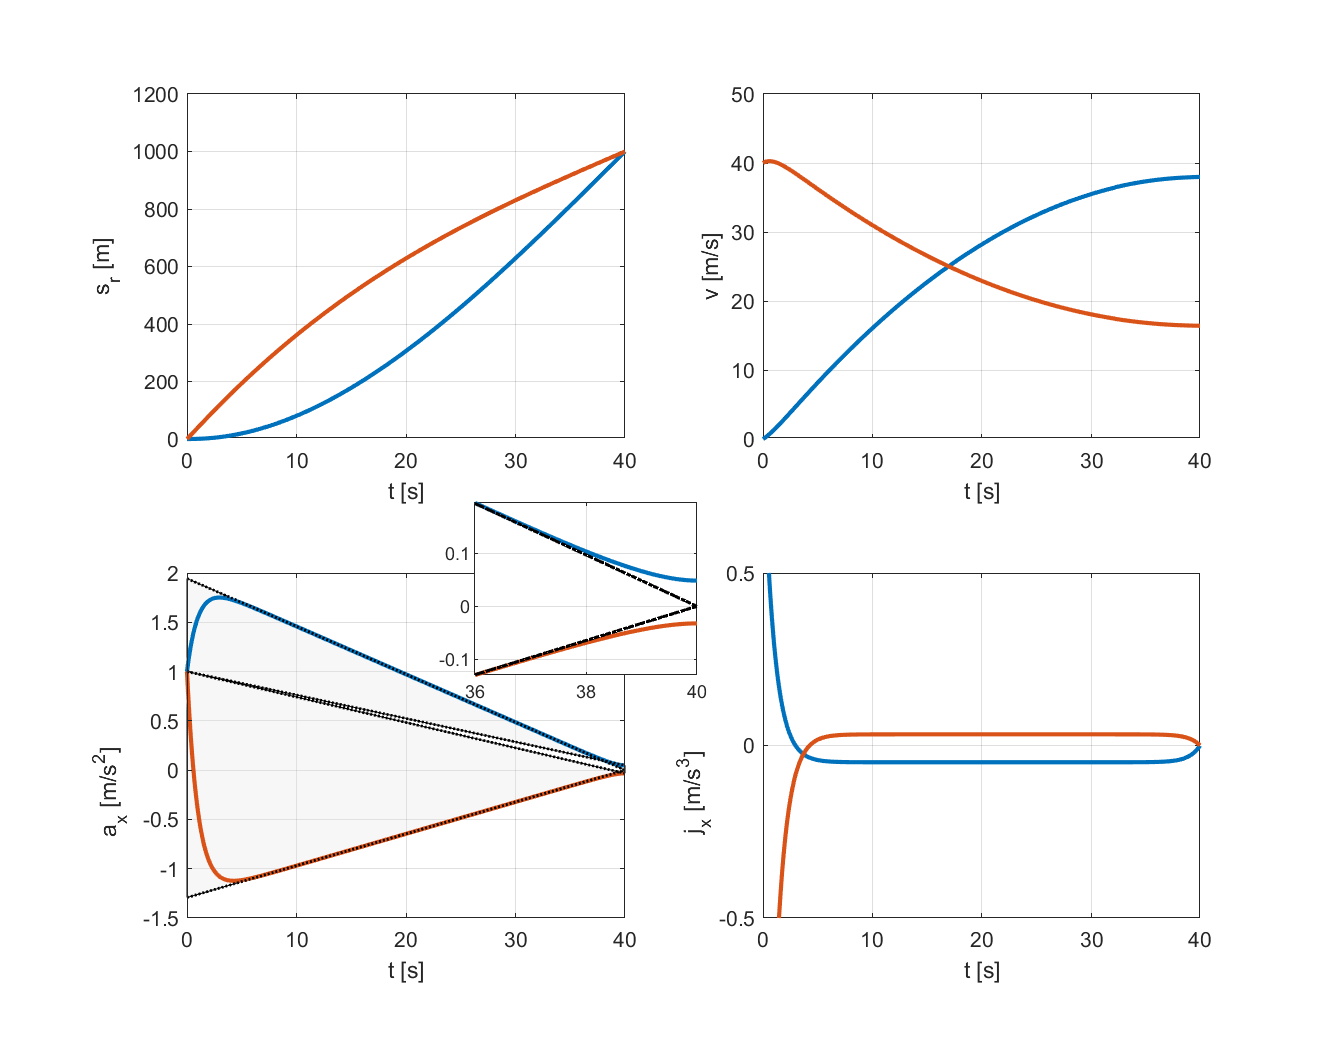
\includegraphics[width=\linewidth]{./Bilder/Ergebnisse/Geradeausfahrt/vf_af_frei_mit_zoom.eps}
	\caption{Lösungstrajektorien der Fahrzeugzustände und der Stellgröße bei einer langen Geradeausfahrt mit $s_f=\valunit{1000}{m}$ und freier Endgeschwindigkeit und -beschleunigung. Der Endzeitpunkt beträgt $t_f = \valunit{40}{s}$.}
	\label{fig:vf_af_frei}
\end{figure} 
In der Abbildung sind die optimalen Zustands- und Stellgrößentrajektorien für unterschiedliche Anfangsgeschwindigkeiten gezeigt, sodass der Ruck und die Beschleunigung jeweils einmal von unten und von oben gegen die Approximation in Bereich zwei konvergieren. Der kleine Ausschnitt in der Mitte der Abbildung gehört zum Graph der Beschleunigung unten links und zeigt den vergrößerten Abschnitt im Bereich von \valunit{36}{s} bis \valunit{40}{s}. Dabei wird deutlich, dass der Endwert der Beschleunigung jeweils außerhalb der durch die Verbindungsgerade und den linearen Anteil der Beschleunigungstrajektorie eingeschlossenen Fläche liegt und damit streng genommen außerhalb der Beschränkung. Da diese Verfehlung allerdings nur einen geringen Einfluss hat, lässt sich der lineare Anteil trotzdem zumindest als Näherungslösung für die Beschränkung verwenden. Zudem zeigt die Abbildung die beiden Nullstellen von $j_x$ und damit Extremstellen von $a_x$, von denen eine jeweils bei liegt.

\subsubsection{Begrenzung des Längsrucks}
Nachdem eingehend erläutert wurde, inwiefern sich aus der analytischen Lösung der Trajektorien Beschränkungen für die Längsbeschleunigung ableiten lassen, sollen nachfolgend Beschränkungen für den Längsruck bei der Geradeausfahrt berücksichtigt werden. Während sich für den Längsruck als Stellgröße über die Kopplung an $\lambda_3$ zwar indirekt ein Endwert vorgeben lässt, kann entgegen der Fahrzeugzustände $s_r, v$ und $a_x$ für $j_x$ allerdings kein Anfangswert vorgegeben werden. Aufgrund dessen ist es möglich, dass die optimale Trajektorie trotz der Bestrafung im Gütefunktional hohe Anfangswerte für $j_x$ liefert. Um dies zu vermeiden, lässt sich der Längsruck mithilfe von Stellgrößenbeschränkungen, die durch das Maximumprinzip von Pontryagin berücksichtigt werden können (siehe Abschnitt \ref{subsubsec:Maximumprinzip} und \ref{subsec:Anwendung_Maximumprinzip}), auf dem gesamten Optimierungsintervall begrenzen. Um den Einfluss der Stellgrößenbeschränkung und den dadurch ermöglichten Komfortgewinn zu veranschaulichen, wird nachfolgend nochmals die lange Geradeausfahrt, diesmal jedoch unter Berücksichtigung von Begrenzungen für den Längsruck untersucht. Im Sinne der Vergleichbarkeit werden die Randbedingungen und Parameter genauso gewählt, wie in Abschnitt \ref{subsubsec:Begrenzung_ax}. Zusätzlich werden verschiedene Maximal- bzw. Minimalwerte für den Längsruck gewählt. Es gilt in jedem Fall $j_{x,\textrm{min}} = -j_{x,\textrm{max}}$. In Abbildung \ref{fig:vf_af_frei_stellgroessenbeschr} sind die optimalen Ruck- und Beschleunigungstrajektorien für die Falle $j_x$ ist unbeschränkt, $j_{x,\textrm{max}} = \valunit{1}{\frac{\unit{m}}{\unit{s^3}}}$ und $j_{x,\textrm{max}} = \valunit{0{,}3}{\frac{\unit{m}}{\unit{s^3}}}$ dargestellt. Aufgrund der freien Endbeschleunigung gilt die Randbedingung $j_x(t_f) = 0$, sodass die Stellgrößenbeschränkung nur zu Beginn der Optimierung aktiv ist. 
\begin{figure}[h] 
	\centering
	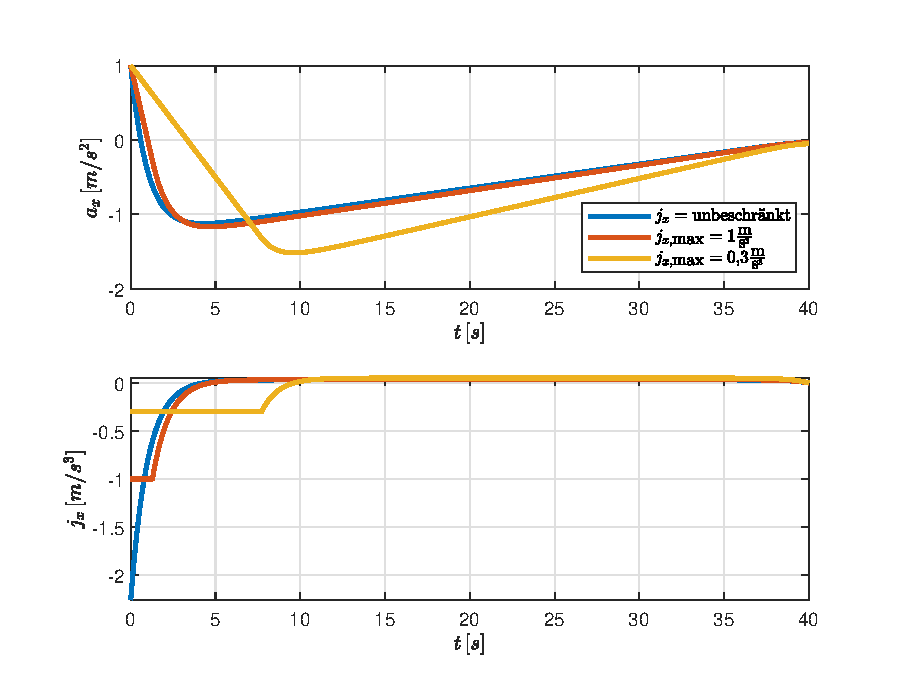
\includegraphics[width=0.8\linewidth]{./Bilder/Ergebnisse/Geradeausfahrt/vf_af_frei_stellgroessenbeschr_ax_und_jx.eps}
	\caption{Ruck- und Beschleunigungstrajektorien bei einer langen Geradeausfahrt mit $s_f=\valunit{1000}{m}$ und freier Endgeschwindigkeit und -beschleunigung unter Berücksichtigung einer Stellgrößenbeschränkung für $j_x$. Der Endzeitpunkt beträgt $t_f = \valunit{40}{s}$.}
	\label{fig:vf_af_frei_stellgroessenbeschr}
\end{figure} 
Die Abbildung macht deutlich, dass sich der maximale Ruck mithilfe der Stellgrößenbeschränkung stark reduzieren lässt. Bei gleicher Endzeit $t_f = \valunit{40}{s}$ geschieht diese Reduktion jedoch auf Kosten einer höheren Maximalverzögerung, da der insgesamt niedrigere Ruck für eine längere zeit auf dem Minimalwert gehalten werden muss, wodurch $a_x$ letztendlich stärker aufintegriert wird. Zudem gehorchen die optimalen Trajektorien nun nicht mehr den in Abschnitt \ref{subsec:Lösungsraum_ax_jx} hergeleiteten Gleichungen. Dennoch bietet die Beschränkung des Rucks eine wirkungsvolle Methode zur Komfortsteigerung. Vergleicht man die Fälle $j_x$ ist unbeschränkt und $j_{x,\textrm{max}} = \valunit{1}{\frac{\unit{m}}{\unit{s^3}}}$ miteinander, lässt sich feststellen, dass die aktive Stellgrößenbeschränkung eine Reduktion des Rucks um \valunit{55{,}76}{\%} bezogen auf den Minimalwert im unbeschränkten Fall bewirkt, während die maximale Verzögerung lediglich um \valunit{3{,}8}{\%} ansteigt. Die weitere Begrenzung des Rucks bedeutet eine Reduktion um \valunit{86{,}73}{\%} bezogen auf den unbeschränkten Fall, während die Verzögerung um insgesamt \valunit{34{,}94}{\%} ansteigt. Bezogen auf die Extremwerte ist damit die Komfortsteigerung des Längsrucks prozentual gesehen mehr als doppelt so hoch wie der Komfortverlust, der gleichzeitig in der Längsbeschleunigung in Kauf genommen werden muss. 
%Abschließend lässt sich festhalten, dass die analytischen Lösungen der optimalen Trajektorien für die Geradeausfahrt sowohl für ein rein energieoptimales Gütefunktional als auch für ein Gütefunktional mit zusätzlicher Bestrafung der Längsbeschleunigung bestimmt werden können und die verbleibenden Unbekannten mithilfe der Randbedingungen des \gls{OP} durch Lösung eines nichtlinearen Gleichungssystems berechnet werden können. Außerdem lässt sich unter Zuhilfenahme einiger Annahmen eine Abschätzung für die Beschränkung der Längsbeschleunigung treffen, über die wiederum Aussagen über den erwarteten Fahrkomfort getroffen werden können. Während der Anfangswert des Längsrucks nicht vorgegeben werden kann, sodass unter Umständen hohe Ruckwerte zu Beginn auftreten können, lässt sich der Endwert des Rucks bei freier Endbeschleunigung über die Endbedingung $\lambda_3(t_f) = 0$ vorgeben. 

\subsection{Heranfahren an eine Ampel bei bekannter Rotphase}\label{subsec:Ampelszenario}
Die Erkenntnisse über den Lösungsraum bei einer Geradeausfahrt mit beschleunigungs- und ruckoptimalem Gütefunktional werden nachfolgend verwendet, um das Heranfahren an eine Ampel mit bekannter Rotphase zu analysieren. Neben der Analyse des Anhalte- bzw. Anfahrvorgangs unter dem Aspekt des Fahrkomforts, dient dieses Szenario auch dem Vergleich zwischen vorausschauender Planung über die Ampelüberquerung hinaus und der weniger vorausschauenden zwei geteilten Planung bis zur Ampel und von dort aus bis zum Zielpunkt. Letzteres entspricht dabei dem vom Menschen gewählten Planungsverhalten, wobei die vorausschauende Variante einige Vorteile bietet. 

Das beschriebene Szenario kann als Geradeausfahrt interpretiert werden, bei der sich das Fahrzeug zu einem bestimmten Zeitpunkt $t_1$ an der Ampel befinden soll. Der Ort, an dem sich die Ampel befindet, kann dabei als die vom Startpunkt der Optimierung aus zurückzulegende Strecke $s_1$ betrachtet werden. Damit ein solches Szenario realistisch umsetzbar ist, muss die Strecke $s_1$ vom Fahrzeug bis zur Ampel, sowie der Zeitpunkt $t_1$ bekannt sein. Dieser wird als der Moment interpretiert, in dem die Ampel von rot auf grün springt und damit das Überqueren der Ampel für das Fahrzeug erlaubt ist\footnote{Ein Ansatz wie der Verkehrsfluss mithilfe von Fahrzeug zu Ampel Kommunikation und adaptiver Ampelphasen in Abhängigkeit des Verkehrsaufkommens verbessert werden kann, wurde in \cite{Gradinescu} untersucht.}. Das Szenario lässt sich dann mithilfe der internen \gls{GNB} $s_r(t_1) = s_1$ bei festem und bekanntem $t_1$ beschreiben. Alternativ kann das Szenario als zwei zusammengesetzte Geradenabschnitte verstanden werden, die an dem über die Zeit und die Strecke definierten Punkt $\mathcal{P}_1 = (t_1, s_1)$ miteinander verknüpft sind. Die Systemdynamik bleibt in den beiden Zeitabschnitten unverändert. Wird die insgesamt benötigte Zeit $t_f$ als Komfortkriterium verwendet, um möglichst schnell zum Zielort zu gelangen, dann kann das Szenario als ein Gesamtoptimierungsproblem mit der internen \gls{GNB} betrachtet werden, wobei $t_f$ über das gesamte Szenario bei der Optimierung berücksichtigt wird. Alternativ kann das Szenario auch als zwei seperate \gls{OP} formuliert werden, wobei das zweite \gls{OP} auf dem ersten aufsetzt, während bei den beiden Problemformulierungen nur das Verhalten im jeweiligen Zeitabschnitt $t_0 \leq t \leq t_1$ bzw. $t_1 \leq t \leq t_f$ berücksichtigt wird. Es sei an dieser Stelle darauf hingewiesen, dass die beiden Herangehensweisen, das Problem zu formulieren, nicht äquivalent sind und daher nicht zu erwarten ist, dass sie identische Ergebnisse liefern. Sie dienen aber der Unterscheidung zwischen dem erwarteten menschlichen Verhalten und dem maschinellen Verhalten eines automatisierten Fahrzeugs, was durch eine einfache Optimierung mit Blick auf das Gesamtintervall erreicht werden kann.

\subsubsection{Vorausschauende Planung}\label{subsubsec:Vorausschauend}
Zunächst soll die vorausschauende Planung des Heranfahrens an die Ampel untersucht werden. Das \gls{OP} für dieses Szenario kann wie folgt formuliert werden
\begin{align}
\min_{\ve{u}} \quad & J(\ve{x},\ve{u},t,t_f) = t_f + \int_{t_0}^{t_f}\frac{1}{2}\fjx j_x^2 + \frac{1}{2}\fax a_x^2~\dtint{t} \\
\textrm{u.B.v.} \quad& \xoftzero = \xzero \\
& s_r(t_1) = s_1 \label{eq:srt1_gleich_s1}\\
& s_r(t_f ) = s_f\,,
\end{align}
wobei die Endzeit frei ist und als Optimierungsvariable betrachtet wird, während der Zeitpunkt $t_1$, zu dem die Ampel überquert werden soll, als fest betrachtet wird. Bis auf die festgelegte Zielstrecke $s_f$ sind die Endzustände frei. Das Ziel dieser Optimierung ist demnach, die Strecke $s_f$ möglichst schnell zurückzulegen unter Berücksichtigung der bekannten Ampelphase und des Fahrkomforts. Die Forderung nach Stetigkeit der Fahrzeugzustände im Übergangspunkt $\mathcal{P}_1$ führt zur Stetigkeitsbedingung 
\begin{equation}
\xoftoneminus = \xoftoneplus
\end{equation}
und schließlich zu der ersten Weierstrass-Erdmannschen-Eckenbedingung (siehe Kapitel \ref{sec:InterneGNB})
\begin{align}
2\tilde{\nu} - \lambda_1(t_1^-) + \lambda_1(t_1^+) &= 0\\
\lambda_2(t_1^-) + \lambda_2(t_1^+) &= 0\\
\lambda_3(t_1^-) + \lambda_3(t_1^+) &= 0\,. \label{eq:l3tminus_l3tplus}
\end{align}
Da $t_1$ fest ist, fällt die zweite Weierstrass-Erdmannschen-Eckenbedingung weg. Im Gegensatz zum menschlichen Planungsverhalten wird die vorausschauende Planung durch die Tatsache definiert, dass das Überqueren der Ampel am Punkt $\mathcal{P}_1$ über eine \gls{GNB} berücksichtigt wird, während die Gesamtzeit $t_f$ bei der Optimierung berücksichtigt wird.

\subsubsection{Menschliche Planung}\label{subsubsec:Mensch}
Bei der menschlichen Planung hingegen lässt sich das \gls{OP}, welches das selbe Gesamtziel hat -- die Strecke $s_f$ unter Berücksichtigung der Ampelphase möglichst schnell zurückzulegen -- in zwei Teilprobleme unterteilen. Für das Gesamtproblem gilt
\begin{equation}
\min_{\ve{u}} \, J(\ve{x},\ve{u},t,t_f) = \min_{\ve{u}} \, J_1(\ve{x},\ve{u},t,t_1) + \min_{\ve{u}} \, J_2(\ve{x},\ve{u},t,t_2)\,.
\end{equation}
Die Teilprobleme $J_1$ und $J_2$ lassen sich dabei wie folgt formulieren:
	\begin{align}
	\min_{\ve{u}} \quad & J_1(\ve{x},\ve{u},t,t_1) = t_1 + \int_{t_0}^{t_1}\frac{1}{2}\fjx j_x^2 + \frac{1}{2}\fax a_x^2~\dtint{t} \\
	\textrm{u.B.v.} \quad & \xoftzero = \xzero \\
	& s_r(t_1) = s_1 
	\end{align}
	\begin{align}
	\min_{\ve{u}} \quad & J_2(\ve{x},\ve{u},t,t_f) = (t_f - t_1) + \int_{t_1}^{t_f}\frac{1}{2}\fjx j_x^2 + \frac{1}{2}\fax a_x^2~\dtint{t} \\
	\textrm{u.B.v.} \quad & \xoftone = \ve{x}_1 \\
	& s_r(t_f) = s_f 
	\end{align}
Diese lassen sich getrennt voneinander lösen und anschließend zur Lösung des Gesamtproblems zusammensetzen. Die Gesamtzeit wird in dieser Art der Problemformulierung also dadurch berücksichtigt, dass die Zeiten der beiden Teilprobleme optimiert werden, wobei das Fahrzeugverhalten für $t>t_1$ im ersten Teilproblem nicht berücksichtigt werden kann und umgekehrt. Der Anfangszustand $\ve{x}_1$ des zweiten Teilproblems entspricht der Lösung des ersten Teilproblems zum Zeitpunkt $t_1$.

\subsubsection{Vergleich der Planungsstrategien}\label{subsubsec:Vergleich}
In Abbildung \ref{fig:svaj_zoomj} sind die optimalen Trajektorien für die beiden erläuterten Planungsstrategien für zwei unterschiedliche Anfangsgeschwindigkeiten mit der Standardparametrierung der Gewichtungsfaktoren dargestellt. Außerdem werden der Ort, an dem die Ampel überquert werden soll und die dazugehörige Zeit, zu $\mathcal{P}_1 = (\valunit{40}{s}, \valunit{350}{m})$ gewählt. Die Gesamtstrecke beträgt $s_f = \valunit{600}{m}$. Wird zunächst nur das Verhalten der vorausschauenden Planung betrachtet (durchgezogene Linien), so fällt ein Unterschied im Beschleunigungsverhalten bzw. im Geschwindigkeitsprofil auf. Startet das Fahrzeug mit einer niedrigen Geschwindigkeit ($v_0 = \valunit{5}{\frac{\unit{m}}{\unit{s}}}$, blaue Linie), beginnt das Fahrzeug sofort zu beschleunigen und die Geschwindigkeit zu erhöhen und überquert die Ampel mit $v(t_1) = \valunit{16{,}78}{\frac{\unit{m}}{\unit{s}}}$. Für den Fall, dass das Fahrzeug bereits mit einer vergleichsweise hohen Geschwindigkeit startet ($v_0 = \valunit{15}{\frac{\unit{m}}{\unit{s}}}$, rote Linie), muss die Geschwindigkeit zunächst gedrosselt werden, damit die Ampel nicht zu früh überquert und damit die Rotphase der Ampel gerissen wird. Die Ampel wird in diesem Fall bei $\mathcal{P}_1$ mit $v(t_1) = \valunit{13{,}02}{\frac{\unit{m}}{\unit{s}}}$, also mit geringerer Geschwindigkeit, passiert. Beim Beschleunigungsverhalten zeigt sich, dass der Betrag der Trajektorie bei einer niedrigeren Startgeschwindigkeit geringere Werte annimmt und daher komfortabler ist im Vergleich zum Starten mit hoher Anfangsgeschwindigkeit. Die niedrigere Startgeschwindigkeit erreicht jedoch nicht nur aus Sicht der Beschleunigung ein höheres Maß an Fahrkomfort. Gleichzeitig lässt sich das Planungsziel schneller erreichen, da das anfängliche Abbremsen nicht notwendig ist und stattdessen von Beginn an gleichmäßig beschleunigt werden kann. In beiden Fällen lässt sich zudem aufgrund der Bedingung \eqref{eq:l3tminus_l3tplus} Stetigkeit für $j_x$ erreichen und so insgesamt ruckarme Lösungen erzielen. Betrachtet man nun die Lösungen bei der menschlichen Planung (gestrichelte Linien), lassen sich die selben qualitativen Zusammenhänge erkennen. Auch bei dieser Art der Planung ist es günstiger mit einer geringeren Geschwindigkeit zu starten, da sich das Ziel dadurch schneller erreichen lässt und geringere Beschleunigungen benötigt werden. Vor allem fällt jedoch auf, dass aufgrund der zwei getrennten Planungen, die bis auf den Anfangszustand unabhängig voneinander sind, in beiden Abschnitten der Anfangsruck nicht vorgegeben werden kann, sodass der Ruck unstetig ist und bei $\mathcal{P}_1$ eine Sprungstelle auftritt. Diese Sprungstelle führt zu deutlich größeren Ruckwerten als bei der vorausschauenden Planung. In \ref{Anhang} ist nochmals der Plot der Stellgröße dargestellt, allerdings mit einer weiteren Achsenskalierung, sodass die kompletten Ruckverläufe inklusive der Überhöhungen an der Sprungstelle zu erkennen sind. Neben der weniger komfortablen Rucktrajektorien, zeigt das Geschwindigkeitsprofil einen weiteren Nachteil der menschlichen Planung gegenüber der vorausschauenden Planung. Das menschliche Verhalten in der weniger vorausschauenden Planung wird damit begründet, dass die Planung abschnittsweise vom Startpunkt bis zur Ampel und von dort bis zum Zielpunkt stattfindet, ohne dass der Abschnitt nach der Ampel im ersten Abschnitt berücksichtigt wird. Dies hat zur Folge, dass die Geschwindigkeit $v(t_1)$ an der Ampel geringer ist, als sie im Idealfall bei vorausschauender Planung sein könnte, weshalb das Fahrzeug bei der menschlichen Planung immer mehr Zeit benötigt, als bei der vorausschauenden Planung.
\begin{figure}[h] 
	\centering
	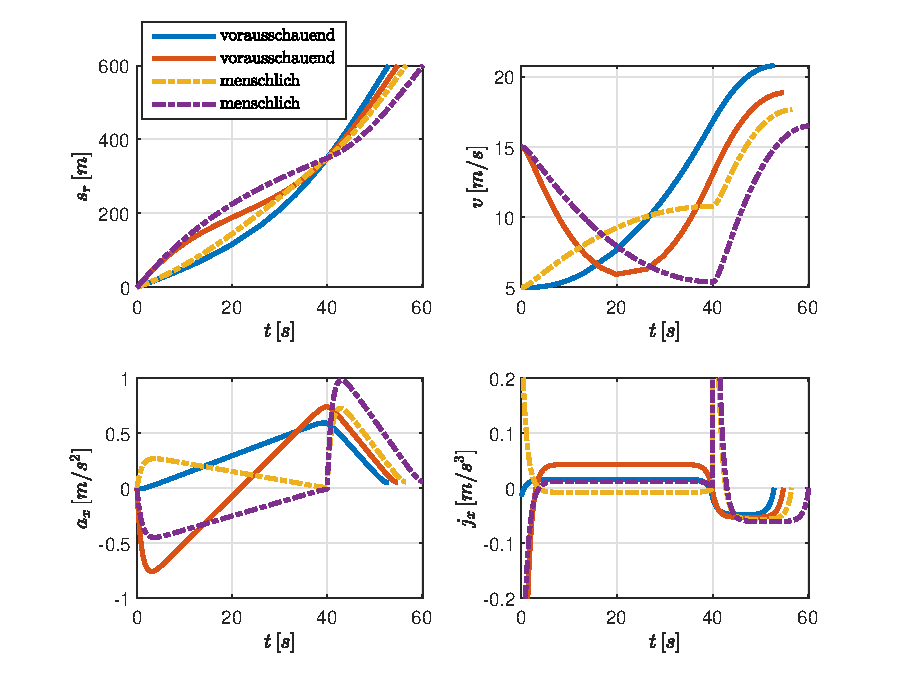
\includegraphics[width=\linewidth]{./Bilder/Ergebnisse/Geradeausfahrt/Ampel/v_5_v_15/svaj_zoomj.eps}
	\caption{Lösungstrajektorien der Fahrzeugzustände und der Stellgröße beim Zufahren auf eine Ampel mit bekannter Rotphase. Darstellung der Ergebnisse für vorausschauende und menschliche (weniger vorausschauend) Planung bei unterschiedlichen Startgeschwindigkeiten.}
	\label{fig:svaj_zoomj}
\end{figure} 

\textbf{Idealer Bremsvorgang}

Als Abschluss dieses Szenarios soll der Blick nochmal speziell auf den Bremsvorgang vor der Ampel bei hohen Anfangsgeschwindigkeiten gerichtet werden. Dazu sind in Abbildung \ref{fig:va_fa_variabel} die Geschwindigkeits- und Beschleunigungsverläufe von vorausschauender und menschlicher Planung für das Szenario mit der höheren Anfangsgeschwindigkeit ($v_0 = \valunit{15}{\frac{\unit{m}}{\unit{s}}}$) gezeigt, allerdings mit unterschiedlichen Gewichtungen \fax~der Beschleunigung. Dabei zeigt sich, dass die Geschwindigkeit bei der menschlichen Planung an der Ampel jeweils am geringsten ist. Dieses Verhalten entspricht dabei am ehesten dem, wie sich eine fahrende Person im Straßenverkehr verhalten würde -- man würde so lange die Geschwindigkeit reduzieren, bis die Ampel schließlich wieder auf grün springt. Bei der vorausschauenden Planung hingegen wird das Minimum deutlich früher erreicht. Dies mag auf den ersten Blick nicht gerade intuitiv erscheinen, da es bedeutet, dass schon stark verzögert wird, obwohl das Fahrzeug noch weit von der Ampel entfernt ist. Zudem bedeutet es, dass bereits beschleunigt wird, bevor die Ampel grün zeigt. Durch diese Weitsicht kann die Ampel allerdings mit höherer Geschwindigkeit überquert und das Endziel schneller erreicht werden. Die vorausschauende Planung mag zwar aus Sicht der Komfortkriterien besser abschneiden, als die menschliche Planung, allerdings ist sie nicht in allen Verkehrssituationen praktikabel. Bei besonders hohem Verkehrsaufkommen, bei dem sich der Verkehr möglicherweise vor einer Ampel staut, ist diese Art der Planung nicht sinnvoll nutzbar, da das Fahrzeug vor der Ampel keine freie Fahrt hat und dadurch nicht schon weit vor der Ampel beschleunigen kann, wie es von der Trajektorie verlangt wird. Zudem würde das starke Abbremsen weit vor der Ampel dazu führen, dass der nachfolgende Verkehr ausgebremst wird.
\begin{figure}[h] 
	\centering
	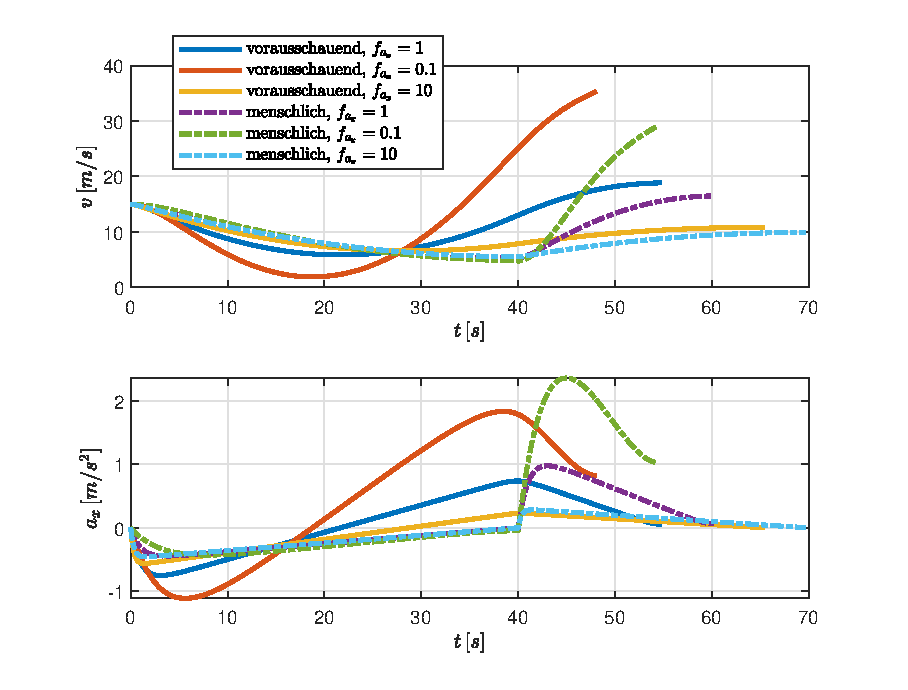
\includegraphics[width=0.9\linewidth]{./Bilder/Ergebnisse/Geradeausfahrt/Ampel/v_5_v_15/va_fa_variabel.eps}
	\caption{Geschwindigkeits- und Beschleunigungstrajektorien für vorausschauende und menschliche Planung für unterschiedliche Gewichtungen der Beschleunigung bei höherer Startgeschwindigkeit.}
	\label{fig:va_fa_variabel}
\end{figure}  

\section{Spurwechsel}\label{sec:Spurwechsel}
Bisher wurde ausschließlich die Längsdynamik des Fahrzeugs bei den untersuchten Szenarien berücksichtigt. Das nachfolgende Szenario Spurwechsel stellt insofern eine Erweiterung der bisher betrachteten Szenarien dar, als dass nun unter Hinzunahme der querdynamischen Größen das Gesamtmodell des Fahrzeugs verwendet wird. Dadurch lassen sich Spurwechsel beschreiben und hinsichtlich der Querdynamik analysieren. 

Bei der Analyse des Spurwechsels werden nachfolgend zwei unterschiedliche Modellbeschreibungen untersucht. Zum einen wird das Fahrzeugmodell mit den Stellgrößen $\ve{u} = [j_x,\,\dot{\kappa}]^T$, wie es in Kapitel \ref{cha:Modellbildung} vorgestellt wurde, verwendet. Zum anderen wird die Systembeschreibung mit $\ve{u} = [j_x,\,\kappa]^T$ betrachtet. Letztere hat aus Sicht des Fahrkomforts den Nachteil, dass der Querruck aufgrund der geringeren Modellordnung in der Querdynamik nicht berücksichtigt werden kann. 

\subsection{Formulierung des Optimierungsproblems}\label{subsec:Gütefunktional_Spurwechsel}
Zunächst wird die Problemformulierung und das daraus resultierende Gütefunktional für die detailliertere Modellbeschreibung erläutert. Der Spurwechsel lässt sich ähnlich wie das zuvor analysierte Ampel-Szenario durch eine Geradeausfahrt mit einer internen \gls{GNB} beschreiben und kann daher wieder in zwei Abschnitte unterteilt werden. Zusätzlich kommt beim Spurwechsel jedoch noch eine Parameteränderung hinzu, die über eine Diskontinuität in der Systembeschreibung berücksichtigt werden kann, wobei die Diskontinuität streng genommen nicht die eigentlich Fahrzeugdynamik betrifft, sondern das Gütefunktional und damit die adjungierten \gls{DGL} verändert. Das \gls{OP} lässt sich wie folgt formulieren:
\begin{align}
\min_{\ve{u}} \quad J(\ve{x},\ve{u},t,t_1) &= t_f + \int_{t_0}^{t_f}\frac{1}{2}\fdr(d_r - d_{\textrm{off}})^2 + \frac{1}{2}\fjx j_x^2 + \frac{1}{2}\fax a_x^2 + \frac{1}{2}\fjy j_y^2 + \frac{1}{2}\fay a_y^2~\dtint{t} \\
\textrm{u.B.v.} \quad \xoftzero &= \xzero \\
s_r(t_1) &= s_1 \\
s_r(t_f) &= s_f \\
d_r(t_f) &= d_1 \label{eq:Spurwechsel_Endbedingung_dr}\\
\psi_r(t_f) &= 0 \label{eq:Spurwechsel_Endbedingung_psir}\\
\kappa(t_f) &= 0 \label{eq:Spurwechsel_Endbedingung_kappa}\\
d_{\textrm{off}} &= 0,\quad t<t_1 \label{eq:Spurwechsel_interneGNB_dr_zero}\\
d_{\textrm{off}} &= d_1,\quad t\geq t_1 \label{eq:Spurwechsel_interneGNB_dr_d1}
\end{align}
Neben den komfortrelevanten Größen Ruck, Beschleunigung und Reisezeit, wird im Gütefunktional zusätzlich die seitliche Abweichung von der Referenzkurve bestraft. Dadurch wird erreicht, dass sich das Fahrzeug trotz Querdynamik immer in der Nähe der Referenzkurve befindet, welche auch in diesem Szenario wieder durch eine krümmungsfreie Gerade beschrieben wird. Der eigentliche Spurwechsel wird dadurch erreicht, dass die seitliche Abweichung bezüglich eines vorgegebenen Offsets $d_{\textrm{off}}$ bestraft wird, welcher durch die Gleichungen \eqref{eq:Spurwechsel_interneGNB_dr_zero} und \eqref{eq:Spurwechsel_interneGNB_dr_d1} beschrieben wird und die angesprochene Parameteränderung darstellt. Durch die Endbedingungen \eqref{eq:Spurwechsel_Endbedingung_dr}--\eqref{eq:Spurwechsel_Endbedingung_kappa} ist gewährleistet, dass die seitliche Abweichung zur neuen Fahrspur sowie der Winkelfehler bezüglich der Referenzkurve verschwinden und sich die Krümmung, die zum Durchführen des Spurwechsels notwendig ist, wieder bei Null einstellt. Die Forderung nach Stetigkeit der Fahrzeugzustände führt wie bereits beim Ampel-Szenario zur Stetigkeitsbedingung und zur ersten Weierstrass-Erdmannschen-Eckenbedingung. Da beim Spurwechsel die zeitliche Optimalität sowohl für den Endzeitpunkt $t_f$ als auch für den Zeitpunkt der internen Übergangsbedingung erreicht werden soll, wird $t_1$ in diesem Szenario frei gelassen, sodass auch die zweite Weierstrass-Erdmannsche-Eckenbedingung gilt. Bei der reduzierten Systembeschreibung, in der die Krümmung als Stellgröße verwendet wird, lässt sich das Optimalsteuerungsproblem analog formulieren, allerdings fallen dann die Bestrafung des Querrucks im Gütefunktional und die Endbedingung für die Krümmung \eqref{eq:Spurwechsel_Endbedingung_kappa} weg. Nachfolgend werden die Lösungen der optimalen Trajektorien für realistische Spurwechsel auf Autobahnen für beide Systembeschreibungen analysiert.

\subsection{Optimale Spurwechseltrajektorien}\label{subsec:Spurwechseltrajektorien}
Die Startgeschwindigkeit des Spurwechsels wird zu $v_0 = \valunit{30}{\frac{\unit{m}}{\unit{s}}} = \valunit{108}{\frac{\unit{km}}{\unit{h}}}$ gewählt. Die beim Spurwechsel geforderte Querablage entspricht mit $d_{\textrm{off}} = \valunit{3{,}5}{m}$ einer üblichen Fahrstreifenbreite auf Autobahnen \cite{ForschungsgesellschaftfurStraenundVerkehrswesen.2008}. Zudem beginnt der Spurwechsel mit $a_0 = 0$ und $\kappa_0 = 0$ aus einem beschleunigungs- und krümmungsfreien Zustand. Für den Spurwechsel wird eine Gesamtstrecke von $s_f = \valunit{300}{m}$ vorgegeben, wobei nach der Hälfte, also bei $s_1 = \valunit{150}{m}$, nicht mehr der seitliche Abstand bezogen auf den ursprünglichen Fahrstreifen, sondern zum neuen Fahrstreifen im Gütefunktional berücksichtigt wird. Der Spurwechsel für das beschriebene Szenario ist in Abbildung \ref{fig:xy_pos_s300_v30} dargestellt, wobei die gewählten Achsen den globalen $x_g$- und $y_g$-Koordinaten entsprechen und somit der Verlauf des Manövers aus der Vogelperspektive dargestellt ist. Neben den Verläufen der optimalen Trajektorien ist auch die Referenzkurve gezeigt. Dabei ist der Ort, ab dem die Querablage für die Bestrafung der seitlichen Abweichung im Gütefunktional den Referenzwert $d_{\textrm{off}}$ ändert, gut zu erkennen. 
\begin{figure}[h] 
	\centering
	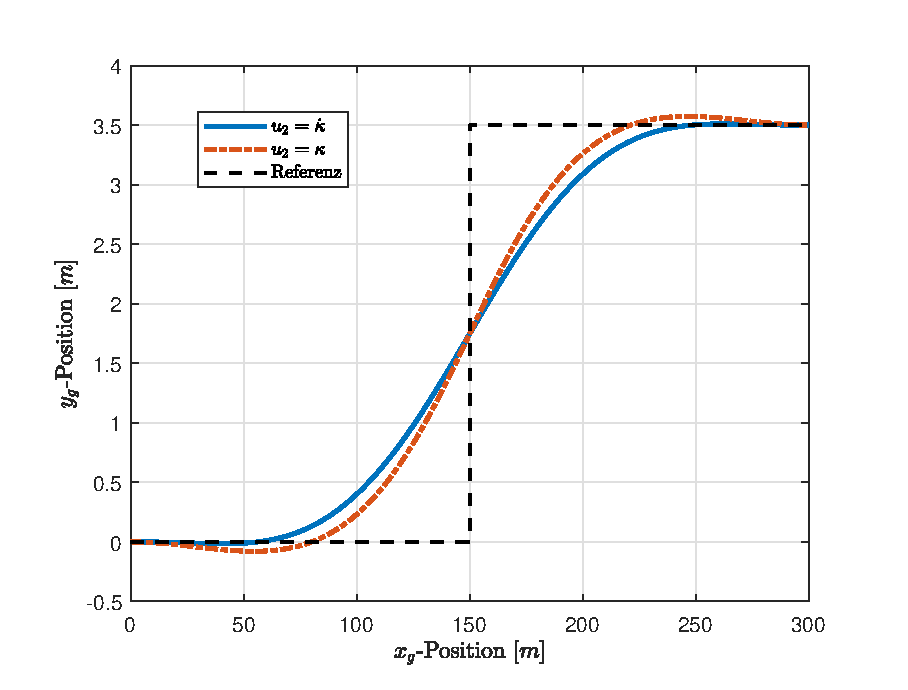
\includegraphics[width=0.7\linewidth]{./Bilder/Ergebnisse/Geradeausfahrt/Spurwechsel/xy_pos_s300_v30.eps}
	\caption{Spurwechseltrajektorien aus der Vogelperspektive für die beiden Modellbeschreibungen unterschiedlicher Ordnung.}
	\label{fig:xy_pos_s300_v30}
\end{figure} 
Zunächst wird die Längsdynamik des Spurwechsels betrachtet. In Abbildung \ref{fig:svaj_s300_v30} sind die Verläufe der Strecke, Geschwindigkeit, Beschleunigung, und des Rucks dargestellt. 
\begin{figure}[h] 
	\centering
	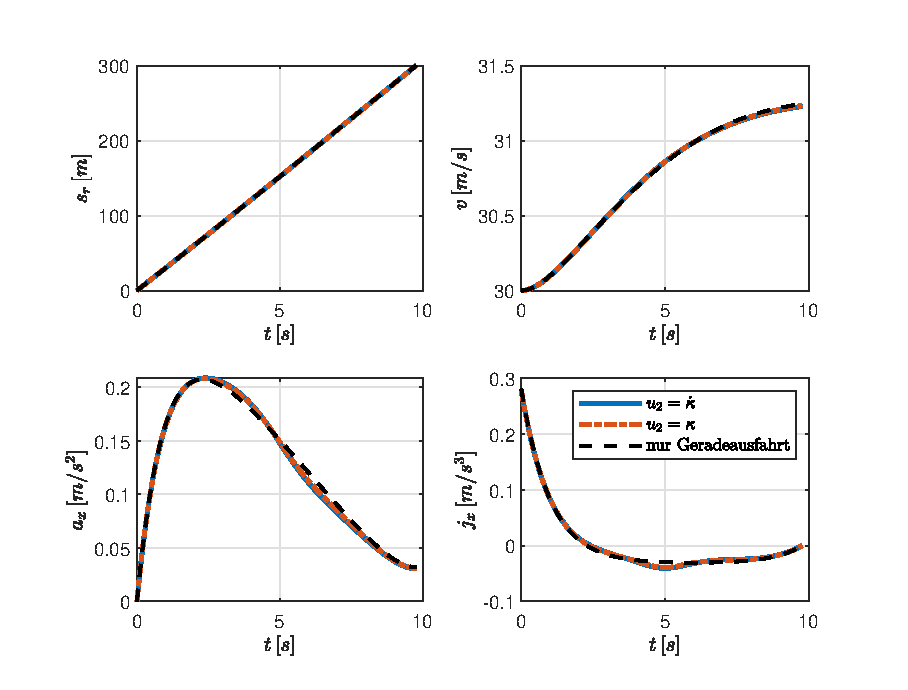
\includegraphics[width=\linewidth]{./Bilder/Ergebnisse/Geradeausfahrt/Spurwechsel/svaj_s300_v30.eps}
	\caption{Trajektorien der Längsdynamik eines Spurwechsels für die beiden Modellbeschreibungen unterschiedlicher Ordnung im Vergleich zur Lösung der Geradeausfahrt ohne Spurwechsel.}
	\label{fig:svaj_s300_v30}
\end{figure} 
Die Abbildung zeigt, dass die unterschiedliche Modellordnung der Querdynamik keinen wesentlichen Einfluss auf die Längsdynamik hat, da die Verläufe nahezu identisch sind. Außerdem ist zu erkennen, dass das längsdynamische Verhalten beim Spurwechsel in guter Näherung dem Verhalten der reinen Geradeausfahrt entspricht, weshalb bei Spurwechseln Längs- und Querdynamik getrennt von einander betrachtet werden können. Dies lässt sich damit begründen, dass das Verhalten bei Spurwechseln durch die Längsdynamik dominiert wird -- während in Querrichtung lediglich eine Strecke von \valunit{3{,}5}{m} zurückgelegt wird, wird bei der hier gewählten Parametrierung in Längsrichtung eine Strecke von \valunit{300}{m} zurückgelegt, sodass dies näherungsweise einer reinen Geradeausfahrt entspricht\footnote{Für dynamischere Spurwechsel, wie sie beispielsweise bei Not- oder Ausweichmanövern auftreten, verliert diese Näherung desto mehr ihre Gültigkeit, je größer der Einfluss der Querdynamik.}. Diese Eigenschaft machen sich die Autoren von \cite{Rathgeber.2016} und \cite{Werling.2011} zu nutze und verfolgen einen Ansatz, bei dem die Quer- und Längsdynamik jeweils als voneinander unabhängige Integratorsysteme betrachtet werden. Dabei ergibt sich ähnlich zur Herleitung in \ref{subsec:Lösungsraum_Geradeausfahrt} für beide Richtungen ein Lösungsraum, der aus Polynomen besteht. Die Berücksichtigung der Querdynamik, so wie sie in dieser Arbeit vorgenommen wird, hat gegenüber dem Ansatz aus \cite{Rathgeber.2016} und \cite{Werling.2011} den Vorteil, dass die Ergebnisse eine höhere Genauigkeit aufweisen, da Längs- und Querdynamik in den \gls{DGL} des Systems miteinander verkoppelt sind. Dafür lässt sich die Lösung der adjungierten \gls{DGL} aufgrund der komplexeren Gleichungen nicht mehr analytisch bestimmen. Die optimalen Trajektorien der querdynamischen Größen zu den zuvor gezeigten Spurwechseln sind in Abbildung \ref{fig:lat_dyn_s300_v30_ohne_dkappa} dargestellt.
\begin{figure}[h] 
	\centering
	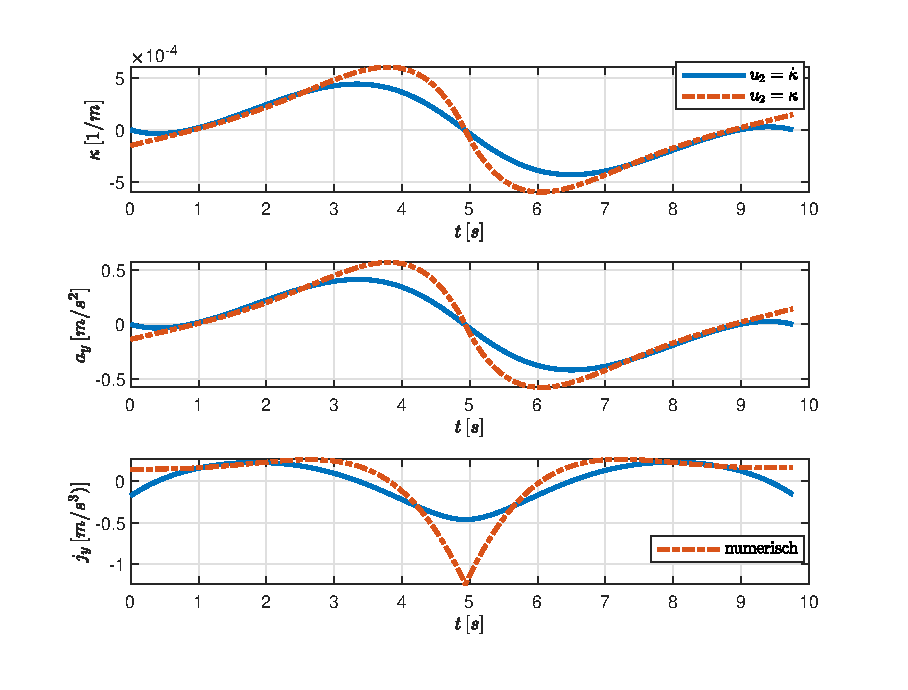
\includegraphics[width=\linewidth]{./Bilder/Ergebnisse/Geradeausfahrt/Spurwechsel/lat_dyn_s300_v30_ohne_dkappa.eps}
	\caption{Trajektorien der Querdynamik eines Spurwechsels für die beiden Modellbeschreibungen unterschiedlicher Ordnung.}
	\label{fig:lat_dyn_s300_v30_ohne_dkappa}
\end{figure} 
Während die Längsdynamik der beiden Modellbeschreibungen identisch modelliert ist und daher auch die Trajektorien nahezu das selbe Verhalten aufweisen, zeigen sich bei der Querdynamik deutliche Unterschiede. Ein wesentlicher Unterschied zeigt sich in den Verläufen der Krümmung. Dadurch, dass $\kappa$ im Modell mit der höheren Ordnung als Zustand betrachtet wird, können sowohl Anfangs- als auch Endwert des Zustands vorgegeben werden, sodass der Spurwechsel aus einem krümmungsfreien und damit auch querbeschleunigungsfreien Zustand begonnen werden kann. Wird $\kappa$ hingegen als Stellgröße verwendet, können keine Anfangswerte vorgegeben werden -- $\kappa$ kann dann lediglich mithilfe des Maximumsprinzips beschränkt werden. Für den Endwert gilt, dass bei der niedrigeren Modellordnung nicht gleichzeitig $\psi_(t_f) = 0$ und $\kappa(t_f) = 0$ gefordert werden können, sodass in dem hier dargestellten Szenario $\kappa(t_f)$ ungleich Null ist. Damit besteht ein Vorteil der höheren Modellordnung darin, dass Randwerte für die Krümmung vorgegeben werden können. Während die optimalen Zeitpunkte für den Übergangspunkt des Spurwechsels $t_1$ und für den Endzeitpunkt $t_f$ bei beiden Modellbeschreibungen identisch sind, lassen sich in den optimalen Verläufen der Beschleunigung und des Querrucks in den unteren beiden Graphen von Abbildung \ref{fig:lat_dyn_s300_v30_ohne_dkappa} sofort qualitative Unterschiede feststellen\footnote{Der Querruck des Spurwechsels bei der niedrigeren Modellordnung mit $u_2 = \kappa$ wird hier durch numerische Differentiation der Querbeschleunigung berechnet.}. Sowohl für den Querruck als auch für die Querbeschleunigung lassen sich komfortablere Trajektorien erzielen, wenn der Querruck zusätzlich bestraft wird. Der Komfortgewinn ist damit zu begründen, dass die Trajektorien beider Größen zum einen niedrigere Werte erzielen und zum anderen weichere Verläufe aufweisen. Es zeigt sich also, dass die Bestrafung des Querrucks nicht nur zu ruckärmeren Trajektorien führt, sondern auch eine Reduktion der Querbeschleunigung bewirkt, obwohl deren Einfluss gegenüber der Optimierung ohne Querruck nicht verändert wurde.

\subsection{Komfortgewinn durch variable Gewichtung der Querabweichung}
Eine Möglichkeit ein höheres Maß an Fahrkomfort zu erzielen, stellt die stärkere Gewichtung der komfortrelevanten Größen dar. Werden die Gewichtungsfaktoren $\fax, \fjx, \fay$ und \fjy~größer gewählt, werden die Verläufe der einzelnen Größen entsprechend flacher, wobei dies auf Kosten der Querabweichung zur Referenzkurve und der Reisezeit geschieht. Eine weitere Möglichkeit zur Beeinflussung des Fahrkomforts bietet die Veränderung der Gewichtung der Querabweichung \fdr. Da sich die Referenzquerablage $d_{\textrm{off}}$ zum Zeitpunkt $t_1$ sprunghaft ändert, lässt sich durch eine stärkere Gewichtung von $d_r$ erreichen, dass der Spurwechsel \glqq schneller\grqq~vollzogen und dadurch dynamischer wird. Eine schwächere Gewichtung hingegen bewirkt genau das Gegenteil, wodurch das Einstellen des seitlichen Versatzes eher gemächlich geschieht. In Abbildung \ref{fig:xy_pos_fdr_var} sind mehrere Spurwechsel für unterschiedliche Gewichtungsfaktoren \fdr~dargestellt, wobei diese das Verhalten der höheren Modellordnung mit $u_2 = \dot{\kappa}$ zeigen. 
\begin{figure}[h] 
	\centering
	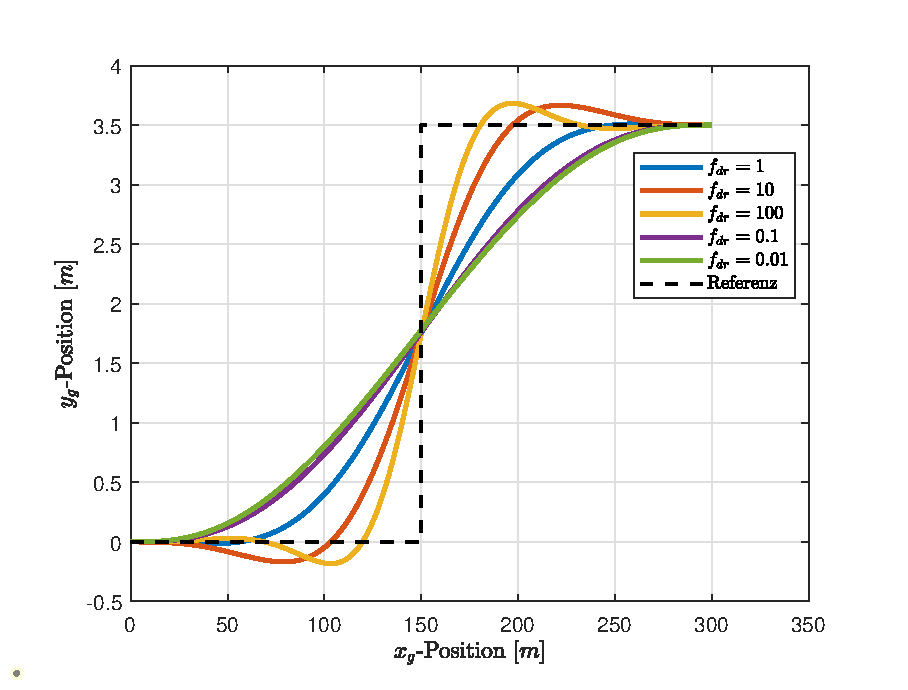
\includegraphics[width=0.7\linewidth]{./Bilder/Ergebnisse/Geradeausfahrt/Spurwechsel/fdr_var/xy_pos.eps}
	\caption{Spurwechseltrajektorien aus der Vogelperspektive für verschiedene Gewichtungen der Querabweichung.}
	\label{fig:xy_pos_fdr_var}
\end{figure} 
Es ist gut zu erkennen, wie die Gewichtung den Verlauf des Spurwechsels beeinflusst -- je höher die Bestrafung, desto steiler ist die seitliche Bewegung, wodurch sich die Trajektorie stärker der sprunghaften Referenzkurve annähert. Dadurch nimmt die Strecke ab, die für das Einstellen des größten Teils der Querablage benötigt wird. Der eigentliche Spurwechsel (abgesehen vom Einschwingverhalten) findet also auf einer kürzeren Strecke statt, wenn die Querabweichung stärker gewichtet wird. Zudem lässt sich erkennen, dass dynamische Spurwechsel mit hoher Bestrafung der Querabweichung ein seitliches Überschwingen aufweisen. Das bedeutet, dass der seitliche Versatz, den das Fahrzeug beim Spurwechsel annehmen soll, kurzzeitig überschritten wird, bis das Fahrzeug am Endpunkt genau den vorgegeben Wert annimmt. Bei sehr hoher Bestrafung kann dies unter Umständen dazu führen, dass Trajektorien entstehen, bei denen das Fahrzeug den Fahrbahnrand kurzzeitig verlassen würde. Derartige Trajektorien wären in der Praxis offensichtlich nicht zulässig. Die zu den Spurwechseln gehörigen Trajektorien der Querdynamik sind in Abbildung \ref{fig:lat_dyn_fdr_var} dargestellt.
\begin{figure}[h] 
	\centering
	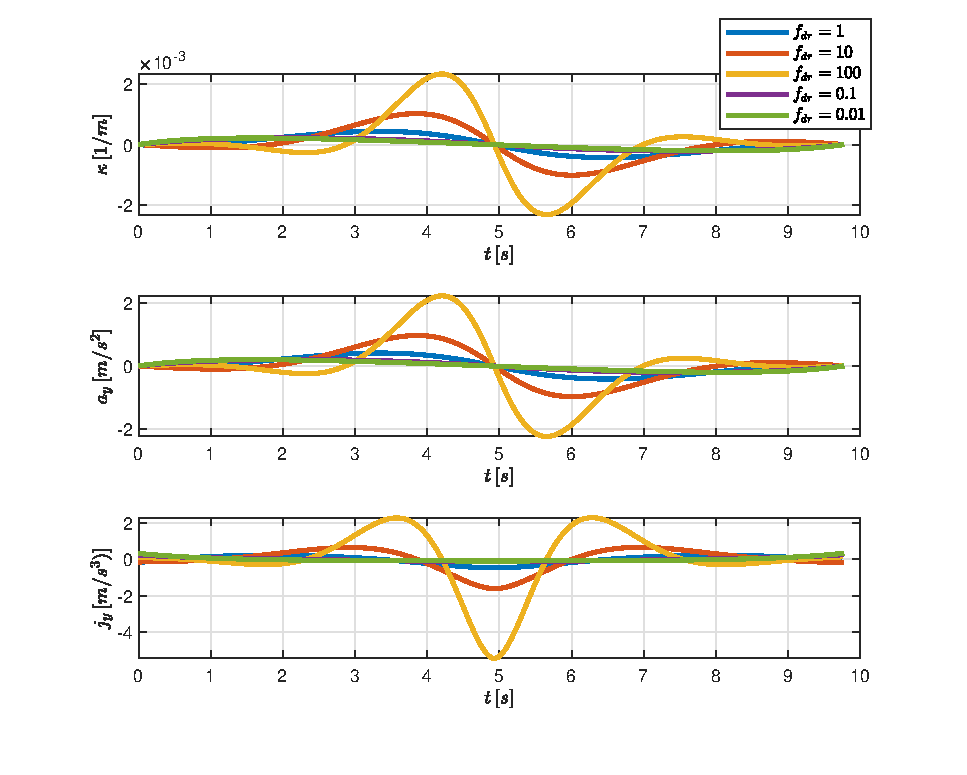
\includegraphics[width=\linewidth]{./Bilder/Ergebnisse/Geradeausfahrt/Spurwechsel/fdr_var/lat_dyn_ohne_kappa.eps}
	\caption{Spurwechseltrajektorien aus der Vogelperspektive für verschiedene Gewichtungen der Querabweichung.}
	\label{fig:lat_dyn_fdr_var}
\end{figure} 
Dabei ist gut zu erkennen, wie die Querdynamik mit zunehmender Bestrafung der Querabweichung zunimmt. Dadurch, dass der Spurwechsel näher an den Verlauf der Referenzkurve gedrückt wird, sind größere Lenkeinschläge bzw. Krümmungen notwendig, weshalb die Querbeschleunigung zunimmt. Da nicht nur größere Krümmungswerte angenommen werden, sondern sich diese bei einer größeren Gewichtung der Querabweichung auch stärker ändern, nimmt zusätzlich der Querruck zu. Damit lässt sich die Aussage treffen, dass der Fahrkomfort des Manövers mit zunehmender Gewichtung der Querabweichung abnimmt. Dieses dynamische Verhalten kann bei einer Sicherheitsbewertung der aktuellen Fahrsituation nützlich sein. Bei freier Fahrt kann ein Spurwechsel beispielsweise mit geringer Bestrafung der Querabweichung geplant werden, da das Manöver mithilfe ruck- und beschleunigungsarmer Trajektorien durchgeführt werden kann und dies zu einem hohen Maß an Komfort führt. Dafür wird allerdings eine weite Strecke benötigt. Wird eine Fahrsituation als sicherheitskritisch eingestuft, wie es bei einem Notausweichmanöver der Fall ist, kann der Spurwechsel mit hoher Bestrafung der Querabweichung geplant werden, da hierbei bis auf das Einschwingen eine deutlich geringere Strecke für das Manöver benötigt wird. Dies geschieht allerdings auf Kosten des Fahrkomforts, wobei dieser in einer Notsituation dem Sicherheitsaspekt unterzuordnen ist. Abschließend ist in Abbildung \ref{fig:svaj_fdr_var} das längsdynamische Verhalten der verschiedenen Spurwechsel dargestellt, und es ist gut zu erkennen, dass die Längsdynamik mit zunehmender Gewichtung der Querabweichung von der stärker werdenden Querdynamik beeinflusst wird. Das dynamische Verhalten des Gesamtsystems wird insbesondere im Bereich um $t_1$ herum von der Querdynamik dominiert. Damit ist auch erkennbar, dass die in \ref{subsec:Spurwechseltrajektorien} erläuterte Näherung, Längs- und Querdynamik getrennt voneinander zu betrachten, nur für Szenarien mit geringer Querdynamik gültig ist.
\begin{figure}[h] 
	\centering
	\includegraphics[width=0.7\linewidth]{./Bilder/Ergebnisse/Geradeausfahrt/Spurwechsel/fdr_var/svaj.eps}
	\caption{Spurwechseltrajektorien aus der Vogelperspektive für verschiedene Gewichtungen der Querabweichung.}
	\label{fig:svaj_fdr_var}
\end{figure} 

\section{Kreisfahrt mit konstanter Krümmung}\label{sec:Kreisfahrt}
Nachdem das Szenario Geradeausfahrt eingehend analysiert und diskutiert wurde, soll nachfolgend das Szenario einer Kreisfahrt untersucht werden. Die Kreisfahrt stellt mit seiner konstanten Krümmung einen vereinfachten Sonderfall einer Kurve dar. Durch die Analyse der Kreisfahrt lassen sich einige Erkenntnisse gewinnen, die später bei der Untersuchung allgemeiner Kurven mit veränderlicher Krümmung, sogenannter Klothoiden, wieder auftauchen.

\subsection{Vernachlässigung der Querdynamik}\label{subsec:Kreisfahrt_ohne_Querdynamik}
Wie in Kapitel \ref{cha:Modellbildung} bereits erklärt, sind die \gls{DGL} des Gesamtsystems unter Berücksichtigung aller Komfortkriterien, der Querdynamik und der von der Strecke abhängigen Referenzkrümmung analytisch nicht lösbar. Aus diesem Grund werden wieder einige Annahmen getroffen, um die Lösung des Optimalsteuerungsproblems zu vereinfachen. Das Kreisfahrtszenario wird zunächst unter Vernachlässigung der Querdynamik bezüglich der Referenzkurve betrachtet. Dazu wird vereinfachend angenommen, dass sich das Fahrzeug immer exakt auf der Referenzkurve mit $\kapparef$ bewegt. Laterale Bewegungen werden dabei vernachlässigt, weshalb nur eine Stellgröße in Längsrichtung benötigt wird. Dafür wird nachfolgend die Längsbeschleunigung mit $u = a_x$ gewählt. Die Querbeschleunigung kann dabei über die Krümmung der Referenzkurve und die Fahrzeuggeschwindigkeit berücksichtigt werden. Das \gls{OP} der Kreisfahrt für das deutlich vereinfachte Modell lässt sich damit wie folgt angeben: 
\begin{align}
\min_{\ve{u}} \quad & J(\ve{x},\ve{u},t,t_f) = t_f + \int_{t_0}^{t_f}\frac{1}{2}\fax a_x^2 + \frac{1}{2}\fay \kapparef^2v^4~\dtint{t} \\
\textrm{u.B.v.} \quad& \xoftzero = \xzero \\
& s_r(t_f ) = s_f\,.
\end{align}
Aus dieser Formulierung folgen die kanonischen \gls{DGL} 
\begin{align}
\dot{s}_r &= v \\
\dot{v} &= a_x \label{eq:dot_v_ax}\\
\dot{\lambda}_1 &= 0 \\
\dot{\lambda}_2 &= -2\fay \kapparef^2v^3 - \lambda_1 \label{eq:dot_l2_Kreisfahrt}
\end{align}
und aus der Steuerungsgleichung folgt
\begin{equation}
	\lambda_2 = -\fax a_x\,. \label{eq:l2_Kreisfahrt}
\end{equation}
\subsubsection{Ruhelage}\label{subsubsec:RL_ohne_Querdynamik}
Dieses System kann schließlich auf Ruhelagen untersucht werden. Dabei stellt sich die Frage, ob es eine Geschwindigkeit \vRL~gibt, die zu einer Ruhelage des Systems führt, welche eine Lösung des Optimalsteuerungsprolems darstellt. Da die Kreisfahrt in der Ruhelage mit konstanter Geschwindigkeit durchfahren werden soll, muss der Zustand $s_r$ bei der Untersuchung aus dem System entfernt werden, sodass sich das reduzierte System mit 
\begin{equation}
\tilde{\ve{z}} = \begin{bmatrix}
v \\
\lambda_1 \\
\lambda_2
\end{bmatrix}
\end{equation}
ergibt. Die konstante Geschwindigkeit führt zudem dazu, dass die Beschleunigung in der Ruhelage Null betragen muss. Nullsetzen von Gleichung \eqref{eq:dot_l2_Kreisfahrt} liefert die Beziehung 
\begin{equation}
\loneRL = -2\fay\kapparef^2\vRL^3\,.
\end{equation}
Diese kann in die Transversalitätsbedingung für freie Endzeit eingesetzt und schließlich nach \vRL~aufgelöst werden. Dabei wird angenommen, dass aufgrund der Ruhelage für alle Größen $v(t_f) = \vRL,...,\lambda_6(t_f) = \lsixRL$ gilt. Aus 
\begin{equation}
H(t_f) = \frac{1}{2}\fax a_x(t_f)^2 + \frac{1}{2}\fay \kapparef^2v(t_f)^4 + \lambda_1(t_f)v(t_f) + \lambda_2(t_f)a_x(t_f) \stackrel{!}{=} -1 
\end{equation}
folgt schließlich
\begin{equation}
\vRL = \sqrt[4]{\frac{2}{3\fay\kapparef^2}} \,. \label{eq:v_RL_ohne_Qerdynamik}
\end{equation}
Damit existiert eine Ruhelage, die eine Lösung des \gls{OP} für die Kreisfahrt mit dem vereinfachten und um $s_r$ reduzierten System darstellt. Die Querbeschleunigung, die sich aus der Referenzkrümmung und der Geschwindigkeit in der Ruhelage berechnen lässt, beträgt
\begin{equation}
\ayRL = \vRL^2\kapparef = \sqrt{\frac{2}{3\fay}} \,. \label{eq:ayRL_Kreisfahrt}
\end{equation}
Die optimale Querbeschleunigung in der Ruhelage bei einer Kreisfahrt ist offensichtlich unabhängig von der durchfahrenen Krümmung und hängt lediglich von der Gewichtung \fay~im Gütefunktional ab.
\subsubsection{\gls{DGL} der Geschwindigkeit}
Mit der Ruhelage des Systems können die Gleichungen noch weiter gelöst werden. Aus \eqref{eq:l2_Kreisfahrt} folgt 
\begin{equation}
\dot{\lambda}_2 = -\fax \dot{a}_x = -\fax \ddot{v}\,. 
\end{equation}
Dieser Zusammenhang kann in Gleichung \eqref{eq:dot_l2_Kreisfahrt} eingesetzt und zu der gewöhnlichen, nichtlinearen \gls{DGL} zweiter Ordnung für die Geschwindigkeit umformuliert werden
\begin{equation}
\ddot{v} = 2\frac{\fay}{\fax}\kapparef^2v^3+\frac{\lambda_1}{\fax}\,, \label{eq:DGL_v_Kreisfahrt_zweite_ordnung}
\end{equation}
wobei für $\lambda_1$ der Wert in der Ruhelage \loneRL~eingesetzt werden kann, da $\lambda_1$ ohnehin konstant ist. Gleichung \eqref{eq:DGL_v_Kreisfahrt_zweite_ordnung} besitzt eine spezielle Form und kann in eine \gls{DGL} erster Ordnung für die Geschwindigkeit umgeformt werden. Mit 
\begin{equation}
	\varphi(v) := 2\frac{\fay}{\fax}\kapparef^2v^3+\frac{\lambda_1}{\fax}
\end{equation}
lassen sich die folgenden Umformungen durchführen.
\begin{align}
	\ddot{v} &= \varphi(v) \\
	2\dot{v} \ddot{v} &= 2\dot{v}\varphi(v)\\
	2\dot{v} \frac{\textrm{d}\dot{v}}{\stkout{\textrm{d}t}} &= 2\frac{\textrm{d}v}{\stkout{\textrm{d}t}}\varphi(v)\\
	(\dot{v})^2 &= \frac{\fay}{\fax}\kapparef^2v^4+2\frac{\lambda_1}{\fax}v + c \label{eq:DGL_v_Kreisfahrt_erste_ordnung}
\end{align}
Diese \gls{DGL} kann auf analytischem Weg nicht gelöst werden, sondern muss mithilfe numerischer Integrationsverfahren (z.B klassisches \gls{RKV}) gelöst werden. Die Integrationsvariable $c$ muss dabei mithilfe der Anfangsgeschwindigkeit $v_0$ und der  Anfangsbeschleunigung $a_{x,0}$ bestimmt werden, wobei letztere nicht vorgegeben werden kann, da $a_x$ die Stellgröße darstellt. Die Anfangsbeschleunigung kann daher beispielsweise durch vorheriges Lösen des Randwertproblems mithilfe des \texttt{bvp4c}-Solvers berechnet werden. Ob die Lösung der Geschwindigkeit ausgehend vom Anfangswert $v_0$ bei der numerischen Integration letztendlich gegen die Ruhelage konvergiert, hängt in hohem Maße vom Anfangswert der Beschleunigung ab, der für die Berechnung der Integrationskonstanten $c$ verwendet wird. In Abbildung \ref{fig:va_bvp4c_vs_odesol} sind die Verläufe der Geschwindigkeit und der Beschleunigung für eine Kreisfahrt von $s_f = \valunit{700}{m}$ bei einer Krümmung von $\kapparef = \valunit{0{,}01}{\frac{1}{\unit{m}}}$ dargestellt. Mit $\fay = 1$ beträgt die Geschwindigkeit in der Ruhelage $\vRL = \valunit{9{,}036}{\frac{\unit{m}}{\unit{s}}}$ und es ist erkennbar, dass die Lösung mittels \texttt{bvp4c}-Solver ausgehend von der Anfangsgeschwindigkeit genau gegen diese Geschwindigkeit konvergiert, während die Beschleunigung gegen Null läuft. Selbiges gilt auch für die Lösung der \gls{DGL} \eqref{eq:DGL_v_Kreisfahrt_erste_ordnung} mittels \gls{RKV}, sofern die Anfangsbeschleunigung $a_{x,0}$ zur Bestimmung der Integrationskonstante $c$ exakt dem Wert der optimalen Lösung entspricht. Bereits kleine Abweichungen von diesem Wert führen dazu, dass die Integration nicht mehr exakt in der Ruhelage mündet und im schlechtesten Fall sogar instabil wird. 
\begin{figure}[h] 
	\centering
	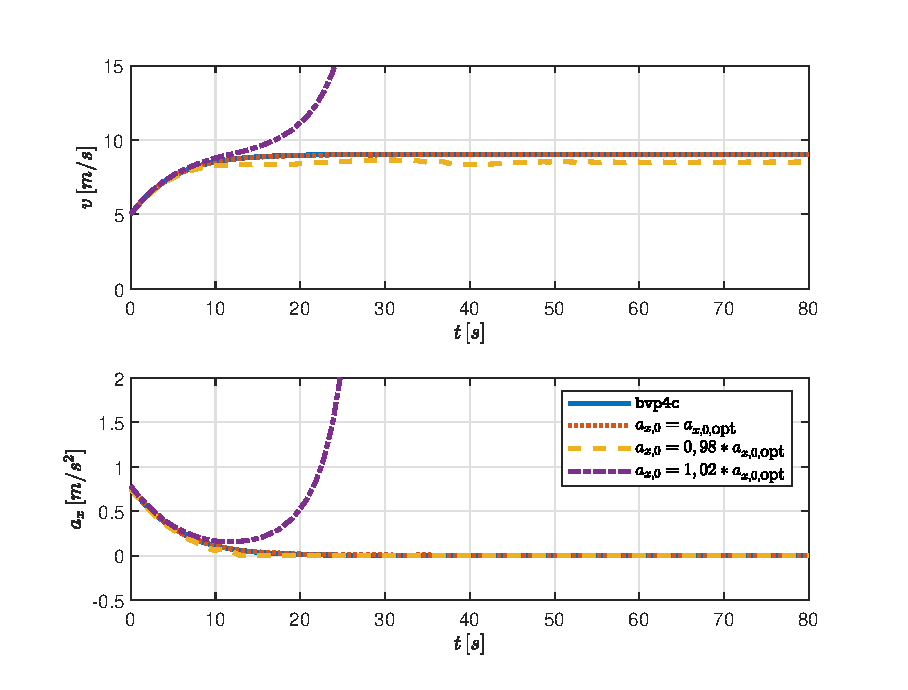
\includegraphics[width=0.8\linewidth]{./Bilder/Ergebnisse/Kreisfahrt/Ohne_Querdynamik/va_bvp4c_vs_odesol.eps}
	\caption{Geschwindigkeit und Beschleunigung einer Kreisfahrt. Vergleich der Lösung mittels \texttt{bvp4c} und Integration der \gls{DGL} \eqref{eq:DGL_v_Kreisfahrt_erste_ordnung} ausgehend von verschiedenen Anfangsbeschleunigungen zur Bestimmung der Integrationskonstante $c$.}
	\label{fig:va_bvp4c_vs_odesol}
\end{figure} 
Diese Abhängigkeit von Anfangwerten, die nicht über die Randbedingungen vorgegeben werden können, ist der Grund, warum eine höhere Ordnung und damit Berücksichtigung des Längsrucks für die Herleitung der Geschwindigkeits-\gls{DGL} ungeeignet ist. Wird das System um den Längsruck als Stellgröße erweitert und dieser im Gütefunktional bestraft, dann lauten die adjungierten \gls{DGL}
\begin{align}
\dot{\lambda}_1 &= 0 \\
\dot{\lambda}_2 &= -2\fay \kapparef^2v^3 - \lambda_1 \\
\dot{\lambda}_3 &= -\fax a_x - \lambda_2\,.
\end{align}
Diese lassen sich mit 
\begin{equation}
\lambda_3 = -\fjx j_x \rightarrow \dot{\lambda}_3 = -\fjx \dot{j}_x = -\fjx \dddot{v}
\end{equation}
wieder ineinander einsetzen, sodass sich schließlich die \gls{DGL} vierter Ordnung für die Geschwindigkeit ergibt
\begin{equation}
\ddddot{v} = \frac{\fax}{\fjx}\ddot{v} - 2\frac{\fay}{\fjx}\kapparef^2v^3 - \frac{\lambda_1}{\fjx}\,. \label{eq:DGL_v_Kreisfahrt_vierte_ordnung}
\end{equation}
Um diese mittels \gls{RKV} zu lösen, müssen die Startwerte für den Ruck sowie dessen Ableitung vorgegeben werden, obwohl diese nicht bekannt sind. Die Formulierung unter Berücksichtigung des Längsrucks ist demnach noch sensitiver gegenüber der Anfangswerte, als die Formulierung ohne den Ruck.

\subsection{Berücksichtigung der Querdynamik}
Nachdem die Kreisfahrt für eine vereinfachte Systembeschreibung ohne Berücksichtigung der querdynamischen Fahrzeugzustände auf Ruhelagen untersucht und eine nichtlineare \gls{DGL} zur Bestimmung der Geschwindigkeitstrajektorie hergeleitet wurde, wird das Fahrzeugmodell für die Kreisfahrt nachfolgend um die querdynamischen Größen erweitert. Dazu wird das System mit den Stellgrößen $\ve{u} = [j_x,\,\dot{\kappa}]^T$ verwendet (siehe Abschnitt \ref{sec:Systemdynamik}) und zunächst nur die Vereinfachung konstanter Referenzkrümmmung mit $\kapparefofs=\kapparefzero$ getroffen. 

\subsubsection{Ruhelage}\label{subsubsec:Ruhelage_Kreisfahrt_mit_Querdynamik}
Analog zum Vorgehen aus Abschnitt \ref{subsubsec:RL_ohne_Querdynamik} wird wieder das um $s_r$ reduzierte System allerdings diesmal mit
\begin{equation}
\tilde{\ve{z}} = 
\begin{bmatrix}
\begin{bmatrix}
v & a_x & d_r & \psi_r & \kappa
\end{bmatrix}^T\\
\begin{bmatrix}
\lambda_1 & \lambda_2 & \lambda_3 & \lambda_4 & \lambda_5 & \lambda_6
\end{bmatrix}^T
\end{bmatrix}
\end{equation}
auf Ruhelagen untersucht. Aus $\dot{\tilde{\ve{z}}} \stackrel{!}{=} 0$ folgt sofort 
\begin{alignat}{2}
	\axRL &= 0 &&\\
	\jxRL &= 0 \rightarrow \lthreeRL &&= 0\\
	\psirRL &= k\pi\,,&&\textrm{mit}~k\in\mathbb{Z}\\
	\dkappaRL &= 0 \rightarrow \lsixRL &&= 0\,,
\end{alignat}
wobei $\psirRL=0$ mit $k=0$ angenommen werden kann, da sich das Fahrzeug weiterhin entlang der Referenzkurve bewegt und daher große Winkelabweichungen nicht vorkommen. Zusätzlich wird unter der Annahme kleiner seitlicher Abweichungen die Vereinfachung $1-d_r\kapparefofs\approx 1$ getroffen, sodass für die Krümmung näherungsweise 
\begin{equation}
	\kappaRL \approx \kapparef \label{eq:kappaRL_approx_kapparef}
\end{equation}
gilt. Durch Einsetzen der bisher bestimmten Ruhelagenwerte in die Gleichungen \eqref{eq:dlambda2}--\eqref{eq:dlambda6} folgt 
\begin{align}
	\loneRL &= -2\fay\kapparef^2\vRL^3\\
	\ltwoRL &= 0\\
	\drRL &= \frac{\kapparef^2\lfiveRL \vRL-\kapparef\loneRL\vRL}{\fdr} \label{eq:dr_RL}\\
	\lfourRL &= 0\\
	\lfiveRL &= -\fay\kapparef \vRL^3\,.
\end{align}
Durch weiteres Umformen lässt sich auch die seitliche Abweichung in Abhängigkeit von \vRL~ausdrücken
\begin{equation}
\drRL = \frac{\fay\kapparef^3\vRL^4}{\fdr}\,.
\end{equation}
Die Geschwindigkeit kann schließlich mithilfe der Transversalitätsbedingung für freie Endzeit bestimmt werden. Diese lässt sich zu der Gleichung
\begin{align}
H(t_f) + 1 &= 0\\
\frac{1}{2}\fdr\drRL^2 - \frac{3}{2}\fay\kapparef^2\vRL^4 + 1 &= 0 \label{eq:Transversalitaet_RL_Kreisfahrt}
\end{align}
zusammenfassen, aus der die Lösung der Geschwindigkeit zu 
\begin{equation}
\vRL = \sqrt[4]{\frac{3\fdr}{2\fay\kapparef^4}-\sqrt{\Big(\frac{3\fdr}{\fay^2\kapparef^4}\Big)^2 - \frac{2\fdr}{\fay^2\kapparef^6}}} \label{eq:v_RL_Kreisfahrt_mit_Querdynamik}
\end{equation}
bestimmt werden kann. Die seitliche Abweichung von der Referenzkurve und dessen Bestrafung spielen bei der Ruhelage unter Verwendung des Systems mit Querdynamik eine besondere Rolle. Die Lösung für \kappaRL~ist nur gültig, wenn die dazugehörige Näherung hinreichend genau erfüllt ist. Dazu muss \drRL~entsprechend klein sein, was nur über eine hohe Bestrafung der Querabweichung erreicht wird. Aus Gleichung \eqref{eq:dr_RL} wird zudem deutlich, dass eine Grenzwertbetrachtung für $\fdr=0$ zu unendlich hohen seitlichen Abweichungen und damit zu einer nicht lösbaren Gleichung \eqref{eq:Transversalitaet_RL_Kreisfahrt} führt, sodass \vRL~in diesem Fall nicht bestimmt werden kann. Eine Ruhelage existiert folglich nur dann, wenn $d_r$ im Gütefunktional bestraft wird. Außerdem sei an dieser Stelle hervorgehoben, dass die Ruhelage, sofern die Parametrierung so gewählt wird, dass diese existiert, nicht exakt auf der Referenzkurve, sondern immer mit seitlichem Versatz \drRL~im Kreisinnern liegt. Eine Verbesserung der Abschätzung von \kappaRL~lässt sich erreichen, indem nachträglich (nachdem \drRL~bestimmt wurde)
\begin{equation}
\kappaRL = \frac{\kapparef}{1-\drRL\kapparef} \label{eq:kappaRL_exakt}
\end{equation}
bestimmt wird. Gleichung \eqref{eq:v_RL_Kreisfahrt_mit_Querdynamik} lässt sich zu 
\begin{equation}
\vRL = \sqrt[4]{\frac{\frac{9\fdr}{2\kapparef^2}-\frac{3}{2}\sqrt{\frac{9\fdr^2-8\fdr\kapparef^2}{\kapparef^4}}}{3\fay\kapparef^2}} \label{eq:v_RL_Kreisfahrt_mit_Querdynamik_umform}
\end{equation}
umformen. Es lässt sich zeigen, dass der Zähler des Wurzelterms dieser Gleichung im für die Krümmung relevanten Bereich $\kapparef\in [-0{,}2~0{,}2]\frac{1}{\unit{m}}$ konstant durch 2 angenähert werden kann, sofern \fdr~groß genug gewählt wird, sodass die Lösung von \vRL~mit dem Ergebnis aus Abschnitt \ref{subsubsec:RL_ohne_Querdynamik} ohne Querdynamik übereinstimmt. Der Zähler des Wurzelterms von Gleichung \eqref{eq:v_RL_Kreisfahrt_mit_Querdynamik_umform} ist in Abbildung \ref{fig:zaehler_vRL} für verschiedene \fdr~dargestellt und es ist gut erkennbar, dass der Verlauf des Zählers im relevanten Bereich näherungsweise konstant ist, wenn \fdr~ausreichend groß ist. Bereits die Gewichtung $\fdr=1$ stellt dabei einen Wert dar, mit dem die erklärte Näherung verwendet und daher \vRL~durch Gleichung \eqref{eq:v_RL_ohne_Qerdynamik} berechnet werden kann. Damit gilt auch für das Modell mit Querdynamik, dass die optimale Querbeschleunigung gemäß Gleichung \eqref{eq:ayRL_Kreisfahrt} berechnet werden kann und nur vom Gewichtungsfaktor \fay~abhängt. Die seitliche Abweichung von der Referenzkurve ist zwar streng genommen kein komfortrelevantes Gütekriterium, allerdings ist die Bestrafung von $d_r$ im Gütefunktional notwendig, damit das Fahrzeug in der Nähe der Referenzkurve bleibt und damit die Ruhelage der Kreisfahrt auch beim Fahrzeugmodell unter Berücksichtigung der Querdynamik existiert.
\begin{figure}[h] 
	\centering
	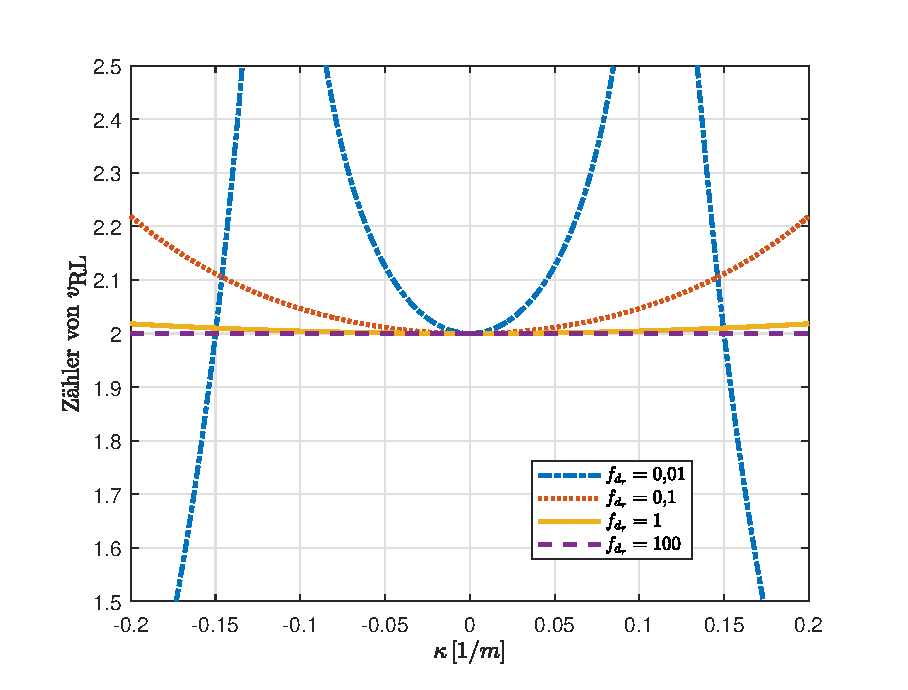
\includegraphics[width=0.7\linewidth]{./Bilder/Ergebnisse/Kreisfahrt/Mit_Querdynamik/zaehler_vRL.eps}
	\caption{Verlauf des Zählers des Wurzelterms von Gleichung \eqref{eq:v_RL_Kreisfahrt_mit_Querdynamik_umform} im Bereich $\kapparef\in [-0{,}2~0{,}2]\frac{1}{\unit{m}}$ für verschiedene $\fdr$.}
	\label{fig:zaehler_vRL}
\end{figure} 

\subsubsection{Linearisiertes Systemverhalten in der Ruhelage}\label{subsubsec:Linearisierung}
Nachdem die Ruhelage des Systems in der Kreisfahrt bestimmt wurde, soll nachfolgend das linearisierte Systemverhalten in der Ruhelage untersucht werden. Dazu werden die kanonischen \gls{DGL} des Gesamtsystems (diesmal wieder mit Berücksichtigung von $s_r$) durch ihre Taylorreihen approximiert, wobei diese nach dem linearen Glied abgebrochen werden \cite{Modellbildung}. Anschließend werden die Taylorreihen durch Einsetzen der Zustands- und Stellgrößen in der Ruhelage ausgewertet, wodurch sich ein lineares System ergibt, welches in der Umgebung der Ruhelage gültig ist \cite{Modellbildung}. Die Strecke $s_r$ kann dabei beliebig gewählt werden. Da die Stellgrößen in Abhängigkeit der Fahrzeugzustände und der adjungierten Zustände ausgedrückt werden können, kann das gesamte linearisierte Systemverhalten durch eine Systemmatrix $\mat{A}$ angegeben werden -- eine Eingangsmatrix wird nicht benötigt. Die Systemmatrix lässt sich dann mittels
\begin{equation}
\mat{A} = \frac{\partial \dot{\ve{z}}}{\partial \ve{z}}
\end{equation}
bestimmen. Aus Gründen der Übersichtlichkeit wird auf die symbolische Berechnung der Systemmatrix an dieser Stelle verzichtet. Die Systemmatrix für das Szenario mit der Standardparametrierung der Gewichtungsfaktoren und $\kapparef = 0{,}01\frac{1}{\unit{m}}$ ist in \ref{appendix:Anhang} angegeben. Die Eigenwerte der Systemmatrix für die Beispielparametrierung in der Laplace-Ebene sind in Abbildung \ref{fig:EW_linear_Kreisfahrt} dargestellt. Dabei liegt der zur Geschwindigkeit und Beschleunigung gehörende Doppelintegratorpol im Ursprung. Die Abbildung zeigt deutlich, dass immer an der Imaginärachse gespiegelte Eigenwerte vorliegen. Dadurch besitzt auch das linearisierte System der Kreisfahrt instabile Eigenmoden. Je nachdem, ob die Endzustände \zoftf~den Werten in der Ruhelage entsprechen, zeigt sich der Einfluss der instabilen Eigenmoden am Ende der Trajektorien. Zudem besitzt das System zwei komplex konjugierte Polpaare, die auf schwingungsfähiges Systemverhalten hindeuten. Diese Schwingungen sind in der Querdynamik des Fahrzeugs deutlich zu erkennen, wenn die Anfangswerte \zzero~nicht der Ruhelage entsprechen.
\begin{figure}[h] 
	\centering
	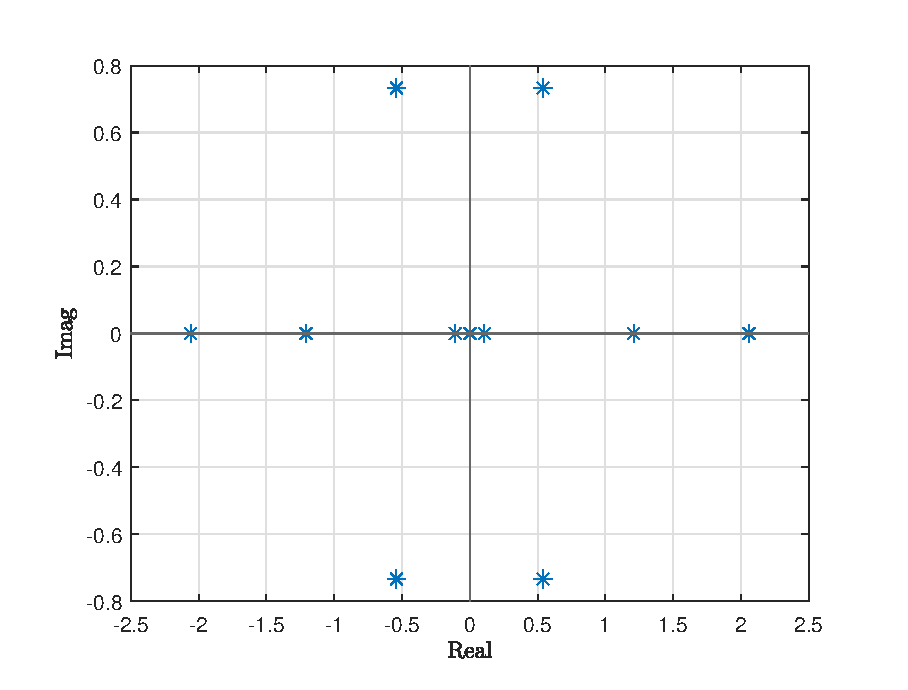
\includegraphics[width=0.7\linewidth]{./Bilder/Ergebnisse/Kreisfahrt/Mit_Querdynamik/EW_linear_Kreisfahrt.eps}
	\caption{Eigenwerte des in der Ruhelage linearisierten Systems mit $\kapparef = 0{,}01\frac{1}{\unit{m}}$.}
	\label{fig:EW_linear_Kreisfahrt}
\end{figure} 
Um dieses Verhalten zu veranschaulichen, sind in Abbildung \ref{fig:Querdyn_RL_ay} die Verläufe der querdynamischen Zustandsgrößen sowie Querbeschleunigung $a_y$ für eine Kreisfahrt von \valunit{500}{m} bei zwei unterschiedlichen Randbedingungen für $d_r$ dargestellt. Zum einen sind die Trajektorien für den Fall gezeigt, dass das System mit $\xzero = \xRL$ in der Ruhelage beginnt (blaue, durchgezogene Linien). In diesem Fall sind außerdem die Endbedingungen $s_r(t_f) = s_f$ und $\psi_r(t_f) = 0$ gewählt. Die restlichen Endzustände -- insbesondere $d_r(t_f)$ -- bleiben frei, sodass die Endwerte der optimalen Trajektorien in der Ruhelage liegen. Der zweite dargestellte Fall beginnt mit $d_{r,0} = 0$, also nicht in der Ruhelage (rote, gestrichelte Linien). Zudem werden die Endbedingungen $s_r(t_f) = s_f, \psi_r(t_f) = 0$ und $d_r(t_f) = 0$ gewählt, sodass das System zum Endzeitpunkt dazu gezwungen wird, die Ruhelage zu verlassen. Die Verläufe verdeutlichen das beschriebene Systemverhalten in Abhängigkeit der Anfangs- und Endbedingungen. Wenn die Optimierung bereits in der Ruhelage startet und die Endbedingungen zulassen, dass auch die Endzustände der Trajektorien der Ruhelage entsprechen, so wird diese über den gesamten Verlauf des Szenarios nicht verlassen --  alle Größen sind konstant. Startet das Fahrzeug jedoch außerhalb der Ruhelage, so wird diese unter Schwingen eingestellt und es zeigt sich der Einfluss der komplex konjugierten Eigenwerte. Sind die Endbedingungen zusätzlich derart vorgegeben, dass ein Beenden der Optimierung außerhalb der Ruhelage erzwungen wird, dann verlässt das Fahrzeug kurz vor Ende des Szenarios die Ruhelage wieder und es werden die vorgegebenen Endzustände eingestellt. In diesem Fall zeigt sich der Einfluss der instabilen Eigenwerte am Ende des Szenarios. Im Graph der Querbeschleunigung unten rechts wird deutlich, dass der Verlauf der Querbeschleunigung in der Nähe der Ruhelage qualitativ dem Verlauf der Krümmung entspricht. Dies liegt daran, dass die Geschwindigkeit in den dargestellten Szenarien nahezu konstant ist. Daher kann \ayRL~als Abschätzung für die zu erwartende Querbeschleunigung verwendet werden. 
\begin{figure}[h] 
	\centering
	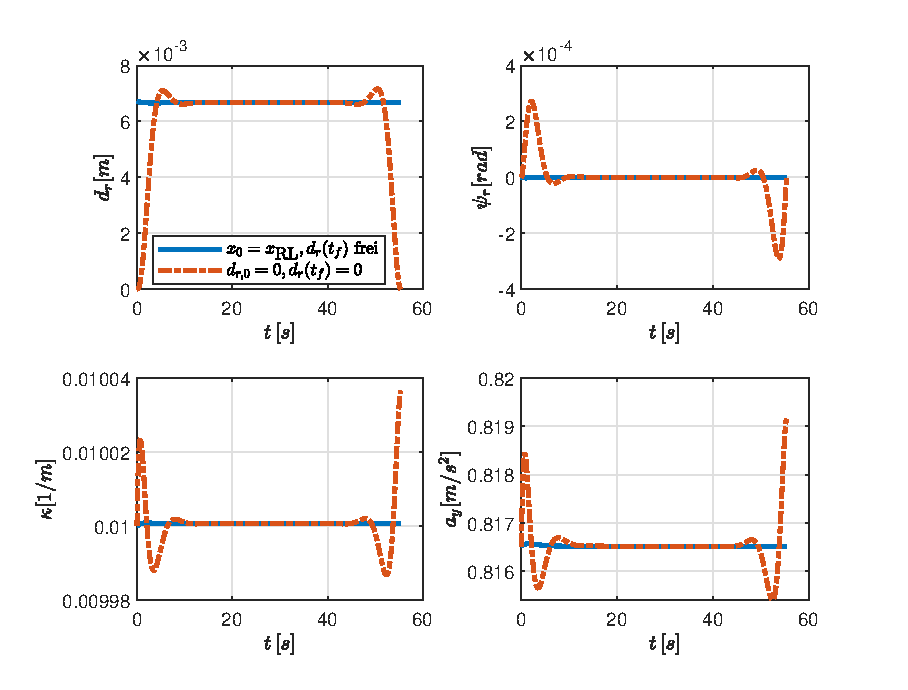
\includegraphics[width=\linewidth]{./Bilder/Ergebnisse/Kreisfahrt/Mit_Querdynamik/Querdyn_RL_ay.eps}
	\caption{Optimale Trajektorien der querdynamischen Größen. Erstens, für den Fall, dass das Fahrzeug in der Ruhelage startet und die Endbedingungen zulassen, dass die Endzustände in der Ruhelage liegen. Zweitens, für den Fall, dass das Fahrzeug \textbf{nicht} in der Ruhelage startet und $d_r(t_f) = 0$ gewählt wird. Die zurückzulegende Strecke beträgt $s_f = \valunit{500}{m}$.}
	\label{fig:Querdyn_RL_ay}
\end{figure} 

Die Kreisfahrt wurde als Sonderfall einer Kurve zunächst ausgehend von einem vereinfachten Modell unter Vernachlässigung der Querdynamik eingeführt und dabei die Modellkomplexität des Szenarios stetig gesteigert, bis letztendlich auch die Beschreibung des vollständigen Modells mit Querdynamik für eine konstante Referenzkrümmung analysiert werden konnte. Dabei konnte gezeigt werden, dass das kanonische Gesamtsystem eine Ruhelage besitzt, die eine Lösung des \gls{OP} darstellt, und gegen die die optimalen Trajektorien immer konvergieren. Damit das System die Ruhelage auch tatsächlich erreicht, muss die Kreisfahrt ausreichend lang sein. Außerdem wurde das linearisierte Verhalten des Systems in der Nähe der Ruhelage untersucht und es konnte festgestellt werden, dass das lineare System sowohl schwingungsfähige als auch instabile Eigenwerte besitzt, deren Einfluss sich jeweils zu Beginn und am Ende der Trajektorien zeigt. Dabei spielt die Wahl der Randbedingungen eine entscheidende Rolle. Zudem konnte festgestellt werden, dass die optimale Querbeschleunigung ausschließlich von der Gewichtung \fay~abhängt. Des Weiteren wurde die besondere Bedeutung der Querabweichung für die Kreisfahrt herausgearbeitet. 

\section{Klothoide mit konstanter Krümmungsänderung}\label{sec:Klothoide}
Nachfolgend wird auch die Vereinfachung einer konstanten Referenzkrümmung weggelassen, sodass Kurven in Klothoidenform mit konstanter Krümmungsänderung betrachtet werden können. Dazu wird das vollständige Fahrzeugmodell, so wie es in Kapitel \ref{sec:Systemdynamik} hergeleitet wurde, mit dem Gütefunktional \eqref{eq:J_eingesetzt} verwendet. In Abbildung \ref{fig:xy_pos_klothoide} ist der Verlauf einer Klothoide ausgehend von der Anfangskrümmung $\kapparefzero = 0$ mit dem Klothoidenparameter $A = \valunit{60}{m}$ dargestellt. Diese Parametrierung repräsentiert eine Autobahnausfahrt \cite{ForschungsgesellschaftfurStraenundVerkehrswesen.2008}. Außerdem beträgt die Strecke der Kurve $s_f = \valunit{720}{m}$, sodass das Fahrzeug den gesamten relevanten Krümmungsbereich von $0-\valunit{0{,}2}{\frac{\unit{1}}{\unit{m}}}$ durchfährt. 
\begin{figure}[h] 
	\centering
	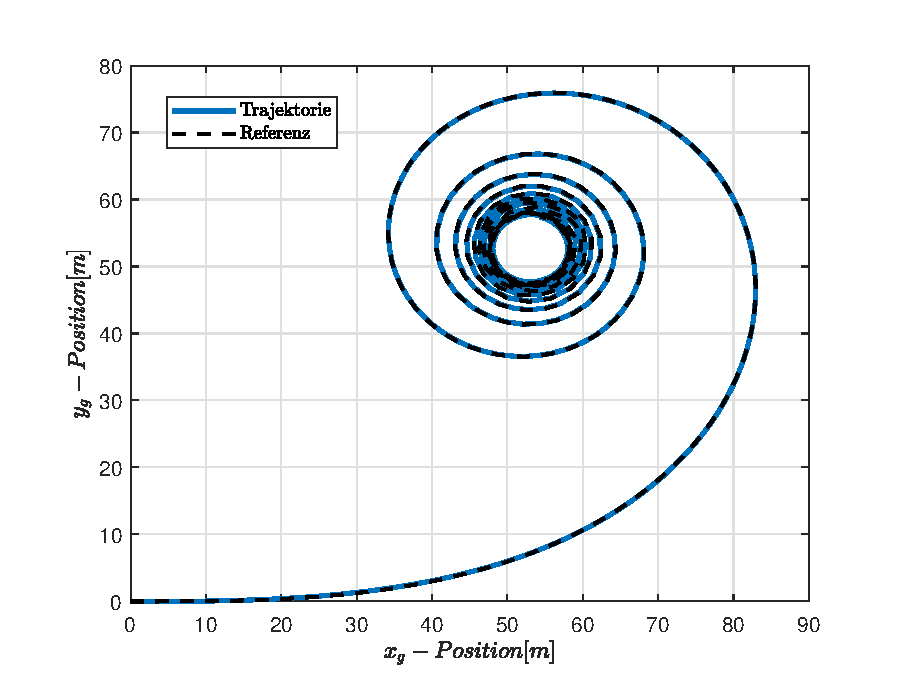
\includegraphics[width=0.7\linewidth]{./Bilder/Ergebnisse/Klothoide/Ohne_umax/xy_pos.eps}
	\caption{Trajektorie einer Kurve in Klothoidenform mit streckenabhängiger Referenzkrümmung aus der Vogelperspektive für die Parametrierung $\kapparefzero = 0,\, A = \valunit{60}{m}$ und $s_f = \valunit{720}{m}$.}
	\label{fig:xy_pos_klothoide}
\end{figure} 
Bei der Kurvenfahrt mit veränderlicher Referenzkrümmung lässt sich feststellen, dass eine Ruhelage für das um $s_r$ reduzierte System analog zur Kreisfahrt nicht bestimmt werden kann. Während bei der Kreisfahrt mit konstanter Referenzkrümmung effektiv keiner der Zustände von $s_r$ abhängt, sodass dieser Zustand einfach aus dem System entfernt werden kann, ist dies bei der streckenabhängigen Referenzkrümmung nicht mehr der Fall. Des Weiteren fällt direkt auf, dass die Referenzkrümmung nun selbst eine zeitliche Abhängigkeit besitzt. Die Dynamik der Referenzkrümmung kann mit 
\begin{equation}
	\dotkapparef = \frac{\dtint{\kapparef}}{\dtint{t}} = \frac{\dtint{\kapparef}}{\dtint{s_r}} \frac{\dtint{s_r}}{\dtint{t}} = \dkapparef \frac{v\cos{\psi_r}}{1-d_r(\dkapparef s_r + \kapparefzero)}
\end{equation} 
angegeben werden. Damit sind die Größen, die vorher in der Ruhelage der Kreisfahrt konstant waren, in diesem Fall zeitlich veränderlich. Allerdings zeigt sich, dass die optimalen Zustands- und Stellgrößentrajektorien der oben dargestellten Klothoide punktweise die Ruhelage der Kreisfahrt annehmen. Mit der Bezeichnung punktweise Ruhelage ist gemeint, dass durch den Verlauf der Referenzkrümmung zu jedem Zeitpunkt eine Ruhelage in Abhängigkeit von \kapparefofs~bestimmt werden kann. Um dies zu veranschaulichen, sind in den Abbildungen \ref{fig:lat_dyn_klothoide} und \ref{fig:svaj_klothoide} die Verläufe der quer- und längsdynamischen Größen beim Durchfahren der oben gezeigten Klothoide dargestellt. Der Graph oben rechts in Abbildung \ref{fig:lat_dyn_klothoide} zeigt die Trajektorie der optimalen Krümmung. 
\begin{figure}[h] 
	\centering
	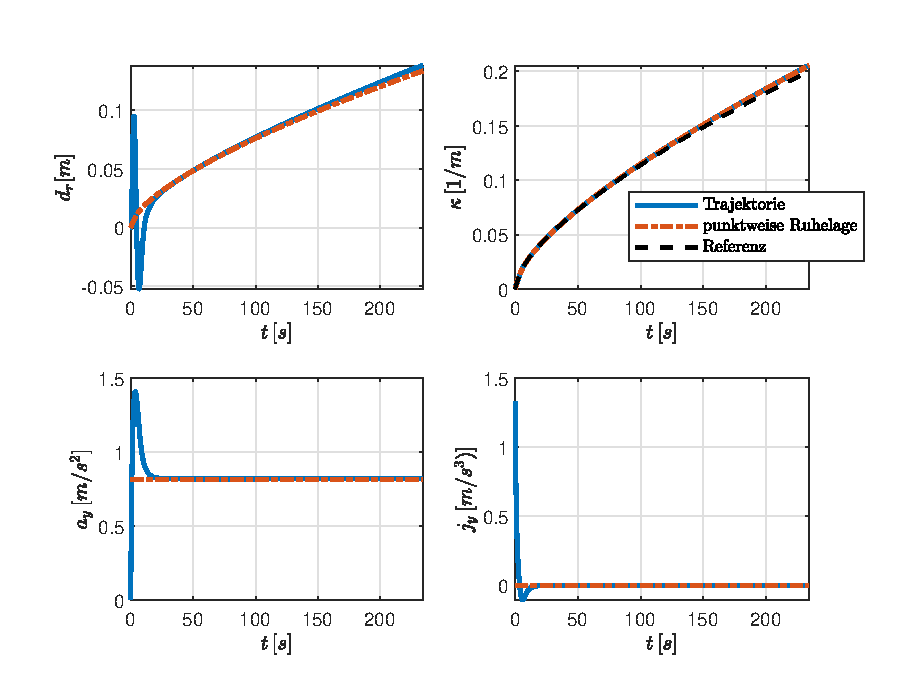
\includegraphics[width=\linewidth]{./Bilder/Ergebnisse/Klothoide/Ohne_umax/lat_dyn.eps}
	\caption{Querdynamik der Klothoide mit $\kapparefzero = 0,\, A = \valunit{60}{m}$ und $s_f = \valunit{720}{m}$.}
	\label{fig:lat_dyn_klothoide}
\end{figure} 
Die punktweise Ruhelage, die ebenfalls dargestellt ist, entspricht dabei der \glqq verbesserten\grqq~Abschätzung gemäß Gleichung \eqref{eq:kappaRL_exakt}. Der Graph zeigt, dass der Verlauf der optimalen Krümmung genau mit dem Verlauf der punktweisen Ruhelage übereinstimmt. Außerdem wird deutlich, dass die Abschätzung \eqref{eq:kappaRL_approx_kapparef} für zunehmende Krümmung stärker von der optimalen Trajektorie abweicht, als die verbesserte Abschätzung. Oben links ist der Verlauf der Querabweichung $d_r$ dargestellt und es ist wie bereits bei der Kreisfahrt das schwingungsfähige Verhalten zu Beginn der Kurvenfahrt zu erkennen. Nachdem die Schwingungen abgeklungen sind, nimmt auch die Querabweichung den Verlauf der punktweisen Ruhelage an. Dabei ist jedoch zu erkennen, dass die optimale Trajektorie von $d_r$ mit zunehmender Krümmung von der punktweisen Ruhelage abweicht. Während die Ruhelage der Kreisfahrt bei einer Krümmung von $\kapparef = \valunit{0{,}2}{\frac{\unit{1}}{\unit{m}}}$ einen Wert von $\drRL = \valunit{0{,}1333}{m}$ annimmt, liefert die optimale Trajektorie einen Wert von $d_{r,\textrm{opt}} = \valunit{0{,}1379}{m}$, was einen Fehler von \valunit{3{,}3358}{\%} bezogen auf den optimalen Wert ergibt. Daraus folgen zweierlei Erkenntnisse: Zum einen liegt die maximale Querabweichung, die während einer Kreisfahrt mit der maximalen Krümmung von \valunit{0{,}2}{\frac{\unit{1}}{\unit{m}}} unter Verwendung der Standardparametrierung der Gewichtungsfaktoren im stationären Zustand erreicht wird, bei unter \valunit{14}{cm}. Dadurch befindet sich das Fahrzeug auch bei den engsten Kurvenradien immer in der Nähe der Referenzkurve. Zum anderen ist der prozentuale Fehler bei der Berechnung von \drRL, der über den gesamten Krümmungsbereich durch die Vereinfachungen bei der Kreisfahrt entsteht (siehe Abschnitt \ref{subsubsec:Ruhelage_Kreisfahrt_mit_Querdynamik}) so gering, dass diese Annahmen für alle relevanten Krümmungen zulässig sind. Der Graph unten rechts in Abbildung \ref{fig:lat_dyn_klothoide} zeigt schließlich, dass der Querruck auch für das Durchfahren einer Klothoide asymptotisch gegen Null konvergiert. Da für den Querruck bei der Lösung des \gls{OP} aufgrund des Zusammenhangs mit der Stellgröße $\dot{\kappa}$ kein Anfangswert vorgegeben werden kann, beginnt dessen Trajektorie mit einem Startwert ungleich Null. Dies ist die Ursache dafür, dass die optimale Querbeschleunigung überschwingt, bevor sie auf einem stationären Wert einschwingt. Der stationäre Endwert der Querbeschleunigung folgt weiterhin Gleichung \eqref{eq:ayRL_Kreisfahrt} und ist daher krümmungsunabhängig, was insofern bemerkenswert ist, als dass sich die optimale Geschwindigkeit und die optimale Krümmung mit dem Verlauf der Strecke verändern. 
\begin{figure}[h] 
	\centering
	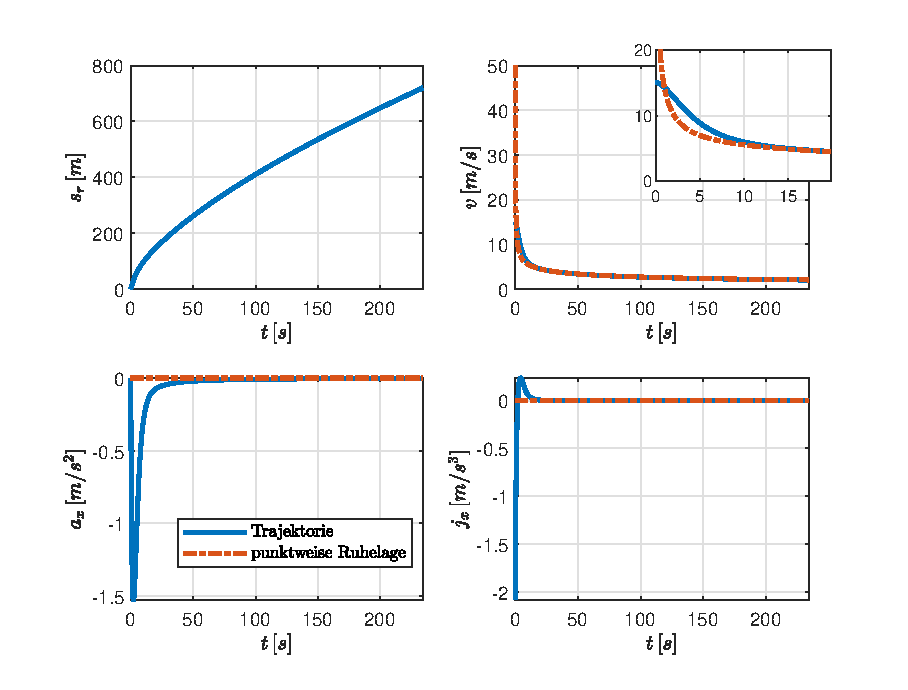
\includegraphics[width=\linewidth]{./Bilder/Ergebnisse/Klothoide/Ohne_umax/svaj.eps}
	\caption{Längsdynamik der Klothoide mit $\kapparefzero = 0,\, A = \valunit{60}{m}$ und $s_f = \valunit{720}{m}$.}
	\label{fig:svaj_klothoide}
\end{figure} 
Im Graph der Geschwindigkeit oben rechts in Abbildung \ref{fig:svaj_klothoide} lässt sich erkennen, dass die Ruhelagengeschwindigkeit für eine Kreisfahrt mit sehr geringer Krümmung gemäß Gleichung \eqref{eq:v_RL_ohne_Qerdynamik} gegen unendlich geht. Da die Anfangsgeschwindigkeit zu $v_0 = \valunit{15}{\frac{\unit{m}}{\unit{s}}}$ gewählt wird, dauert es ca. \valunit{10}{s}, bis die optimale Fahrzeuggeschwindigkeit der punktweisen Ruhelage entspricht. Im weiteren Verlauf der Geschwindigkeitstrajektorie zeigt sich jedoch, dass auch die Geschwindigkeit beim Durchfahren der Klothoide asymptotisch gegen die punktweise Ruhelage geht. Die Längsbeschleunigung und der Längsruck konvergieren wie bereits bei den querdynamischen Größen unter Überschwingen gegen ihren stationären Endwert, wobei dieser für beide Größen bei Null liegt.

\subsection{Begrenzung des Querrucks}
Bei der Geradeausfahrt konnte bereits gezeigt werden, dass sich der Längsruck, für den als Stellgröße kein Anfangszustand vorgegeben werden kann, mithilfe einer Stellgrößenbeschränkung begrenzen lässt, sodass die hohen Ruckwerte am Anfang unterdrückt werden können. Analog dazu soll nachfolgend untersucht werden, inwiefern sich eine ähnliche Begrenzung des Querrucks mithilfe einer Stellgrößenbeschränkung für $\dot{\kappa}$ erreichen lässt. Dazu sind in Abbildung \ref{fig:lat_dyn_klothoide_umax} nochmals die optimalen Trajektorien für die Querdynamik des Fahrzeugs beim Durchfahren der Klothoide für die Fälle unbeschränkte Stellgröße und Beschränkung von $\dot{\kappa}$ dargestellt. Der Längsruck ist dabei in beiden Fällen unbeschränkt und die Parametrierung der Referenzkurve sowie die Anfangszustände des Fahrzeugs bleiben gegenüber der zuvor untersuchten Klothoide unverändert. Die Grenzen der Stellgröße werden zu 
\begin{equation}
	\dot{\kappa}_{\textrm{max}} = \valunit{2{,}5\textrm{e}{-03}}{\frac{\unit{1}}{\unit{m\cdot s}}} \quad\textrm{mit~} \dot{\kappa}_{\textrm{max}} = -\dot{\kappa}_{\textrm{max}}
\end{equation}
gewählt. Der Graph oben rechts in Abbildung \ref{fig:lat_dyn_klothoide_umax} zeigt das Aktivwerden der Stellgrößenbeschränkung, wodurch $\dot{\kappa}$ um etwa die Hälfte des unbeschränkten Maximalwerts reduziert wird. Dies führt zu einem deutlich geringeren Maximum im Querruck, wie der Graph unten rechts verdeutlicht. Diese Reduktion des Querrucks kann als Steigerung des Fahrkomforts interpretiert werden. Der Verlauf des Querrucks zeigt allerdings auch, dass von einem Anschlag der Stellgröße an einer der beiden Grenzen nicht direkt auf den Querruck geschlossen werden kann, da dieser neben $\dot{\kappa}$ noch dem Einfluss weiterer Größen unterliegt (siehe Gleichung \eqref{eq:jy}). Daher kann der Querruck durch eine Beschränkung der Stellgröße zwar reduziert, jedoch nicht im eigentlichen Sinne \glqq beschränkt\grqq~werden. Aus Sicht des Fahrkomforts lässt sich noch eine weitere Verbesserung erkennen. Im unbeschränkten Fall besitzt die Krümmungsänderung keinen Vorzeichenwechsel, weshalb auch die Steigung von $\kappa$ nur ein Vorzeichen besitzt. Dadurch steigt die Krümmung deutlich schneller an, als im beschränkten Fall, sodass die Querbeschleunigung im unbeschränkten Fall ein deutliches Überschwingen aufweist. Im beschränkten Fall hingegen führt die Stellgrößenbeschränkung dazu, dass $\dot{\kappa}$ einen Vorzeichenwechsel besitzt und kurzzeitig die untere Grenze $\dot{\kappa}_{\textrm{min}}$ erreicht. Dieser Vorzeichenwechsel bewirkt ein \glqq Zurücknehmen\grqq~der Krümmung, weshalb diese nicht so schnell ansteigt, wie im unbeschränkten Fall. Dadurch nähert sich die Querbeschleunigung im beschränkten Fall langsam von unten dem stationären Endwert an, ohne dabei überzuschwingen. Auch dieses Verhalten kann als Komfortgewinn eingestuft werden. Durch die Beschränkung der Stellgröße $\dot{\kappa}$ lässt sich also sowohl eine Reduktion der Querbeschleunigung, als auch des -rucks erzielen, was beides zu einer komfortableren Fahrt führt.
\begin{figure}[h] 
	\centering
	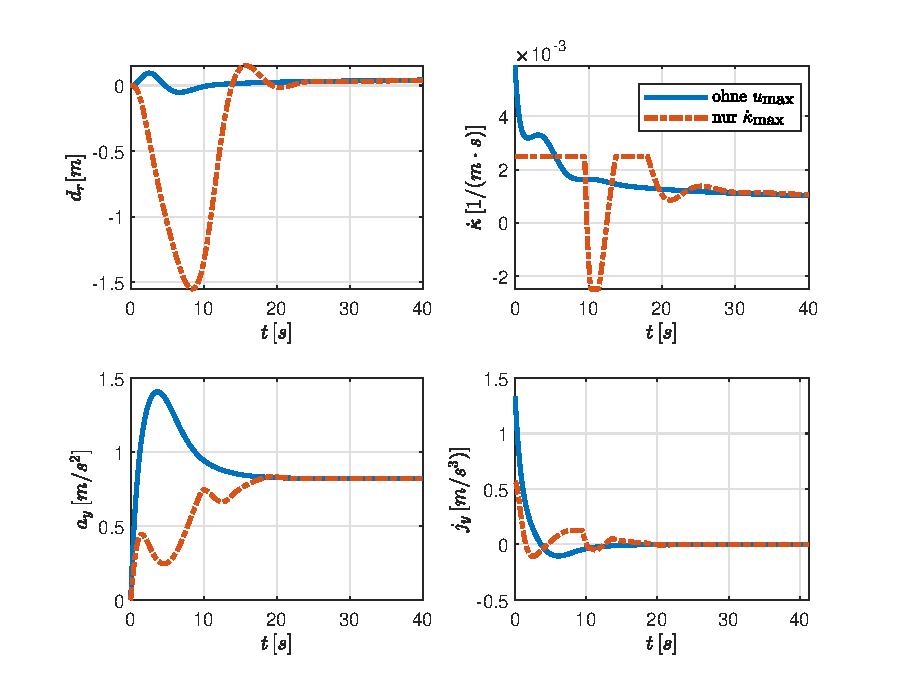
\includegraphics[width=\linewidth]{./Bilder/Ergebnisse/Klothoide/nur_dkappa_max/lat_dyn.eps}
	\caption{Querdynamik der Klothoide unter Verwendung von Stellgrößenbeschränkungen im Vergleich zum unbeschränkten Fall.}
	\label{fig:lat_dyn_klothoide_umax}
\end{figure} 
Der erzielte Komfortgewinn geschieht jedoch auf Kosten der Reisezeit und der Querabweichung. Während die Gesamtzeit, die aus Gründen der besseren Darstellung der Abbildungen in den Graphen nicht dargestellt ist, im unbeschränkten Fall $t_f = \valunit{234{,}04}{s}$ beträgt, verlängert sich die Zeit bei Berücksichtigung der Stellgrößenbeschränkung zu $t_f = \valunit{239{,}32}{s}$. Gemessen an der Gesamtdauer von knapp \valunit{4}{min}, die für das Durchfahren der vollen Klothoide benötigt wird, ist diese Zeiteinbuße jedoch akzeptabel. Bei der Querabweichung hingegen führt die Beschränkung von $\dot{\kappa}$ zu deutlich größeren Abweichungen, wie oben links zu erkennen ist. Die Beschränkung der Krümmungsänderung kann als Beschränkung der Lenkwinkeländerung des Fahrzeugs interpretiert werden. Durch die aktive Stellgrößenbeschränkung reicht das verfügbare Maximum der Lenkwinkeländerung nicht aus, um der Krümmungsvorgabe der Referenzkurve zu folgen. Dadurch wird die Referenzkurve verfehlt und es entsteht eine größere seitliche Abweichung. Sobald die unbeschränkte Stellgröße die obere Grenze $\dot{\kappa}_{\textrm{max}}$ wieder unterschreitet, kann der entstandene Fehler ausgebessert werden, indem die Stellgröße des beschränkten Systems länger auf dem Maximum gehalten wird. Dies wiederum führt dazu, dass die Krümmung durch Integration von $\dot{\kappa}$ zeitweise den Referenzwert überschreitet, was den zuvor beschriebenen Vorzeichenwechsel in der Krümmungsänderung von $\dot{\kappa}_{\textrm{max}}$ zu $\dot{\kappa}_{\textrm{min}}$ erklärt. Die zum Teil deutlich größere seitliche Abweichung muss bei der Bewertung, ob eine geplante Trajektorie zulässig ist, berücksichtigt werden, da zu große seitliche Abweichungen von der Referenzkurve zum Verfehlen der Fahrbahn und im schlimmsten Fall zu Kollisionen mit anderen \GenderPl{Verkehrsteilnehmer} führen können.
%Dazu sind in Abbildung \ref{fig:lat_dyn_klothoide_umax} und in Abbildung \ref{fig:svaj_klothoide_umax} nochmals die optimalen Trajektorien für die Quer- und Längsdynamik des Fahrzeugs beim Durchfahren der Klothoide für die Fälle unbeschränkte Stellgröße, Beschränkung nur für $\dot{\kappa}$ und Beschränkung für $\dot{\kappa}$ sowie $j_x$ dargestellt. Die Parametrierung der Referenzkurve bleibt dabei gegenüber Abschnitt \ref{sec:Klothoide} unverändert. Die Grenzen der Stellgrößen werden zu 
%\begin{equation}
%	\ve{u}_{\textrm{max}} = \begin{bmatrix}
%	j_{x,\textrm{max}}\\
%	\dot{\kappa}_{\textrm{max}} 
%	\end{bmatrix} = \begin{bmatrix}
%	\valunit{2}{\frac{\unit{m}}{\unit{s^3}}}\\
%	\valunit{2{,}5\textrm{e}{-03}}{\frac{\unit{1}}{\unit{ms}}}
%	\end{bmatrix}\, \quad\textrm{mit~} \ve{u}_{\textrm{min}} = -\ve{u}_{\textrm{max}}
%\end{equation}
%gewählt. Der Graph oben rechts in Abbildung \ref{fig:lat_dyn_klothoide_umax} zeigt das Aktivwerden der Stellgrößenbeschränkungen, wodurch $\dot{\kappa}_{\textrm{max}}$ um etwa die Hälfte des Maximalwerts im unbeschränkten Fall reduziert wird. Dies führt zu deutlich geringeren Extremwerten im Querruck, wie der Graph unten rechts verdeutlicht. Diese Reduktion des Querrucks kann als Steigerung des Fahrkomforts interpretiert werden. Der Verlauf des Querrucks zeigt allerdings auch, dass von einem Anschlag der Stellgröße an einer der beiden Grenzen nicht direkt auf den Querruck geschlossen werden kann, da dieser neben $\dot{\kappa}$ noch dem Einfluss weiterer Größen unterliegt (siehe Gleichung \eqref{eq:j_y}). Daher kann der Querruck durch eine Beschränkung der Stellgröße zwar reduziert, jedoch nicht im eigentlichen Sinne \glqq beschränkt\grqq~werden. Aus Sicht des Fahrkomforts  
%\begin{figure}[h] 
%	\centering
%	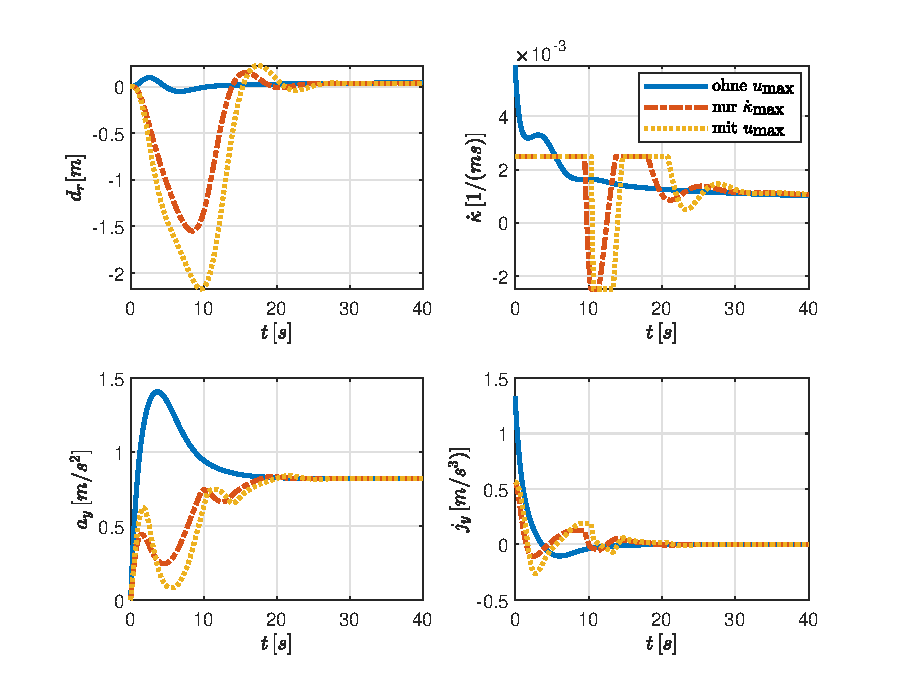
\includegraphics[width=\linewidth]{./Bilder/Ergebnisse/Klothoide/Mit_umax/lat_dyn.eps}
%	\caption{Querdynamik der Klothoide unter Verwendung von Stellgrößenbeschränkungen im Vergleich zum unbeschränkten Fall.}
%	\label{fig:lat_dyn_klothoide_umax}
%\end{figure} 
%\begin{figure}[h] 
%	\centering
%	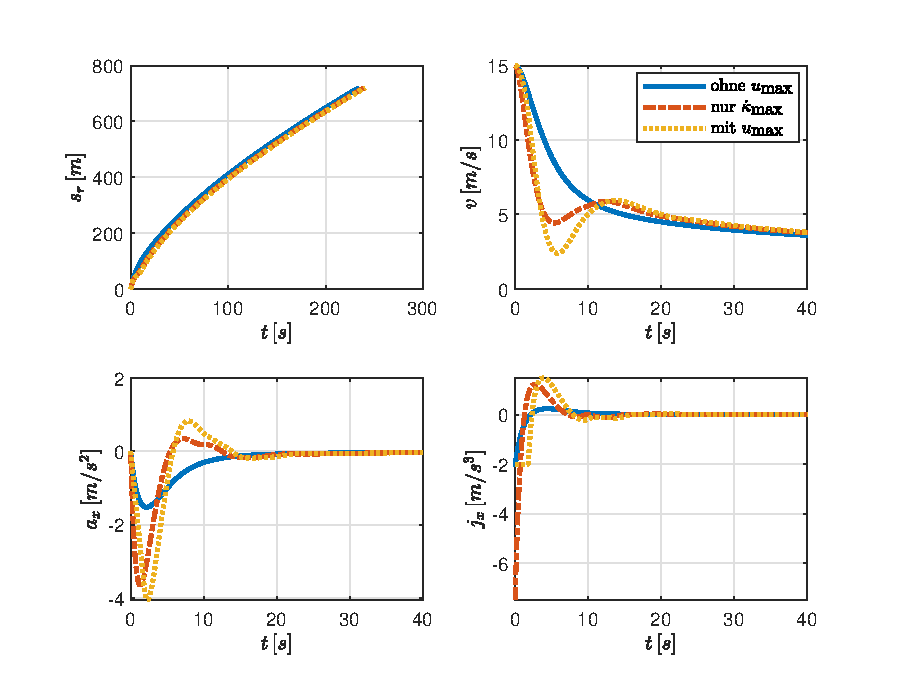
\includegraphics[width=\linewidth]{./Bilder/Ergebnisse/Klothoide/Mit_umax/svaj.eps}
%	\caption{Längsdynamik der Klothoide unter Verwendung von Stellgrößenbeschränkungen im Vergleich zum unbeschränkten Fall.}
%	\label{fig:svaj_klothoide_umax}
%\end{figure} 
\section{Gerade-Kurve-Gerade-Kombination}
Als Abschluss der Analyse verschiedener Fahrszenarien sollen Gerade-Kurve-Gerade-Kombinationen untersucht werden. Dieses Szenario lässt sich durch Zusammensetzen mehrerer Teilszenarien beschreiben und es stehen dabei vor allem die Übergänge zwischen den einzelnen Teilszenarien im Fokus. Für die Untersuchung werden die unterschiedlichen zuvor eingeführten Möglichkeiten zur Betrachtung einer Kurvenfahrt verwendet und hinsichtlich des Fahrkomforts miteinander verglichen. Dabei handelt es sich um die folgenden alternativen Systembeschreibungen (nachfolgend als \glqq Fälle\grqq~bezeichnet): 
\begin{enumerate}
	\item Kreisfahrt mit konstanter Referenzkrümmung exakt auf der Referenzkurve, Fahrzeugmodell ohne Querdynamik.
	\item Kreisfahrt mit konstanter Referenzkrümmung allgemein entlang der Referenzkurve, Fahrzeugmodell mit Querdynamik.
	\item Kurvenfahrt mit streckenabhängiger Referenzkrümmung allgemein entlang der Referenzkurve, Fahrzeugmodell mit Querdynamik.
\end{enumerate}
\subsection{Formulierung des Optimierungsproblems}
Die Kurve (bzw. der Kreis) in der Mitte des Gesamtszenarios wird derart gewählt, dass eine Drehung um genau \valunit{360}{\degree} erzielt wird. Für alle drei Fälle wird die gesamte zu durchfahrende Strecke zu $s_f = \valunit{500}{m}$ gewählt. Die Strecke der Kurve selbst kann durch die Integration der Referenzkrümmung über der Strecke bestimmt werden
\begin{equation}
	\dtint{s_{r,\textrm{Kurve}}} = \frac{1}{\kappa_{\textrm{ref}}(s_r)}\dtint{\psi_{ref}} \,. \label{eq:Kurvenstrecke}
\end{equation}
Im 3. Fall mit der klothoidenförmigen Kurve wird vor Beginn der Kurve eine Strecke von $s_1 = \valunit{100}{m}$ zurückgelegt. Dadurch, dass die Krümmung bei der Klothoide zunächst zunimmt und anschließend wieder abnimmt, entsteht eine Schleife deren Mittelpunkt gegenüber dem Kurvenanfang leicht in Richtung der $x_g$-Achse verschoben ist. Damit die Kurvenfahrt des 1. und 2. Falls mit dem 3. Fall vergleichbar ist, wird die Referenzkurve von Fall 1 und 2 so parametriert, dass der Kurvenmittelpunkt der Kreisfahrt auf einer Achse liegt mit dem Kurvenmittelpunkt der Klothoide. Dazu beträgt die Strecke, die vor Beginn der Kurve zurückgelegt wird, im 1. und 2. Fall $s_1 = \valunit{156{,}2538}{m}$. Die konstante Referenzkrümmung der Kreisfahrt wird mit $\kapparef = \valunit{0{,}0263}{\frac{\unit{1}}{\unit{m}}}$ derart gewählt, dass der am weitesten von der Geraden entfernte Punkt der Referenzkurve in allen drei Fällen identisch ist. Abbildung \ref{fig:gerade_kurve_gerade_xy_pos} zeigt die optimalen Trajektorien der drei Fälle sowie die Referenzkurven der Klothoide und der Kreisfahrt im globalen Koordinatensystem $\mathcal{F}_g$ aus der Vogelperspektive\footnote{Dadurch, dass die maximale seitliche Abweichung im 2. Fall mit $\valunit{37{,}05}{cm}$ gegenüber der Achsenskalierung gering ist, ist diese in Abbildung \ref{fig:gerade_kurve_gerade_xy_pos} kaum erkennbar, sodass es den Anschein erweckt, als würden die Verläufe von Fall 1 und 2 nahezu übereinander liegen.}. Die Abbildung verdeutlicht dabei die für die Parametrierung der Referenzkurve relevanten Zusammenhänge. 
\begin{figure}[h] 
	\centering
	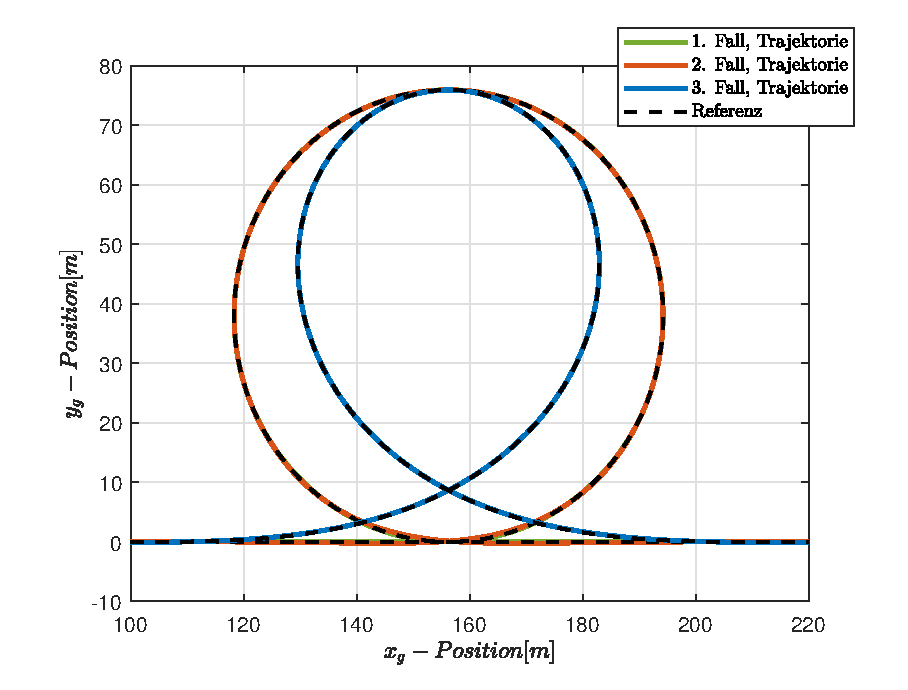
\includegraphics[width=0.7\linewidth]{./Bilder/Ergebnisse/Gerade_Kurve_Gerade/gerade_kurve_gerade_xy_pos.eps}
	\caption{Trajektorien einer Gerade-Kurve-Gerade-Kombination für die drei unterschiedlichen Möglichkeiten zur Beschreibung des Szenarios aus der Vogelperspektive.}
	\label{fig:gerade_kurve_gerade_xy_pos}
\end{figure} 
Da sich das Fahrzeug am Ende des Szenarios wieder in einer Geradeausfahrt befinden soll, werden zusätzlich die Endbedingungen $d_r(t_f) = \psi_r(t_f) = \kappa(t_f) = 0$ gewählt, während die Endgeschwindigkeit $v(t_f)$ und -beschleunigung $a_x(t_f)$ frei bleiben. Die Übergänge zwischen der Kurve und den Geradenabschnitten lassen sich mithilfe interner \gls{GNB} und diskontinuierlicher Systemdynamiken (siehe Abschnitte \ref{sec:InterneGNB} und \ref{sec:Diskontinuität}) beschreiben. Damit lässt sich das Gesamtszenario aus einzelnen Teilszenarien zusammensetzen, wobei die abschnittsweise gültige Systemdynamik hinsichtlich der Referenzkrümmung variiert. Für die Fälle 1 und 2 gilt 
\begin{equation}
\underbrace{\textrm{Gerade}}_{\kappa_{\textrm{ref}} = 0} \quad \rightarrow \quad \underbrace{\textrm{Kreis}}_{\kappa_{\textrm{ref}} = \textrm{konst.}} \quad \rightarrow \quad \underbrace{\textrm{Gerade}}_{\kappa_{\textrm{ref}} = 0} 
\end{equation}
und für den 3. Fall gilt 
\begin{equation}
\underbrace{\textrm{Gerade}}_{\kappa_{\textrm{ref}} = 0} \quad \rightarrow \quad \underbrace{\textrm{Kurvenanstieg}}_{\kappa_{\textrm{ref}} = \dkapparef (s_r-s_1)} \quad \rightarrow \quad \underbrace{\textrm{Kurvenabstieg}}_{\kappa_{\textrm{ref}} = -\dkapparef (s_r-2s_2+s_1)} \quad \rightarrow \quad \underbrace{\textrm{Gerade}}_{\kappa_{\textrm{ref}} = 0} \,.
\end{equation}
Wie man sieht, lässt sich die Gerade-Kurve-Gerade-Kombination der Fälle 1 und 2 durch insgesamt drei Teilszenarien beschreiben, während für den 3. Fall vier Teilszenarien benötigt werden, da die Krümmung der Klothoide nach der Hälfte der Kurve das Vorzeichen wechselt. Das \gls{OP} des Gesamtszenarios für die drei Systembeschreibungen unter Verwendung der jeweiligen Systemdynamik kann als
\begin{align}
\min_{\ve{u}} \quad J(\ve{x},\ve{u},t,t_f) &= t_f + \int_{t_0}^{t_f}\frac{1}{2}\fdr d_r^2 + \frac{1}{2}\fjx j_x^2 + \frac{1}{2}\fax a_x^2 + \frac{1}{2}\fjy j_y^2 + \frac{1}{2}\fay a_y^2~\dtint{t} \\
\textrm{u.B.v.} \quad \xoftzero &= \xzero \\
s_r(t_1) &= s_1 \\
s_r(t_2) &= s_2 \\
(s_r(t_3) &= s_3\,, \quad \textrm{gilt nur für 3. Fall}) \\
s_r(t_f) &= s_f \\
d_r(t_f) &= 0 \\
\psi_r(t_f) &= 0 \\
\kappa(t_f) &= 0
\end{align}
formuliert werden. Neben Gleichung \eqref{eq:Transversalitaet}, die aufgrund der freien Endzeit gilt, muss für die freien Endzustände Gleichung \eqref{eq:Lambdaend} gelten. An den internen Übergangsstellen zwischen den Geradenstücken und der Kurve wird weiterhin die Stetigkeit der Zustände gefordert und es gelten die erste und zweite Weierstraß-Erdmannsche-Eckenbedingung (siehe Gleichungen \eqref{eq:Stetigkeit_t1}--\eqref{eq:WeierstrassErdmann2}). Es sei angemerkt, dass die Bestrafungen der seitlichen Abweichung und des Querrucks für den Fall 1 ohne Querdynamik aus dem Gütefunktional wegfallen, da diese Größen in dieser Systembeschreibung nicht berücksichtigt werden können. Zudem wird die Querbeschleunigung in diesem Fall, wie bereits in Abschnitt \ref{subsec:Kreisfahrt_ohne_Querdynamik}, durch die Referenzkrümmung und die Fahrzeuggeschwindigkeit beschrieben. Für die Gewichtung der Gütekriterien wird die Standardparametrierung verwendet.
\subsection{Optimale Trajektorien}
Nachdem die Verläufe der drei Fälle bezüglich der jeweiligen Referenzkurve sowie die Formulierung des Optimierungsproblems erläutert wurden, sollen nachfolgend die optimalen Trajektorien der Längs- und Querdynamik analysiert werden. In Abbildung \ref{fig:gerade_kurve_gerade_lat_dyn} sind dazu die Trajektorien der Querdynamik dargestellt. Im Graph oben links ist die seitliche Abweichung $d_r$ von der Referenzkurve dargestellt (für die Fälle 2 und 3, da für den Fall 1 keine Querabweichung im Modell berücksichtigt wird). Es ist deutlich zu erkennen, dass das Fahrzeug im Übergang zwischen einem Geradenstück und der Kurve in beiden Fällen seitlich um die Referenzkurve schwingt, um die komfortrelevanten Gütekriterien in den Übergangspunkten -- insbesondere den Querruck -- gering zu halten. Dabei zeigt sich außerdem, dass die seitliche Abweichung unter Verwendung der Klothoide ein insgesamt niedrigeres Niveau hat, als bei der kreisförmigen Kurve, was auf die stetige Zu- bzw. Abnahme der Krümmung zurückzuführen ist. Der Graph oben rechts zeigt die optimalen Krümmungstrajektorien im Vergleich zur Referenzkrümmung. Dabei wird der Unterschied zwischen den Fällen 1/2 und 3 hinsichtlich der Referenzkrümmung deutlich -- in den Fällen 1 und 2 weist die Referenzkrümmung eine sprunghafte Änderung auf, während sie im 3. Fall linear an- und absteigt\footnote{Das lineare Verhalten der Krümmung im 3. Fall gilt bezüglich der zurückgelegten Strecke, allerdings ist im Graph in Abbildung \ref{fig:gerade_kurve_gerade_lat_dyn} der Zeitverlauf der Krümmung dargestellt, weshalb der lineare Zusammenhang nicht exakt zu erkennen ist.}. Da in der Systemdynamik des 1. Falls keine Querdynamik berücksichtigt ist, ist die \glqq optimale\grqq~ Krümmung in diesem Fall identisch zur Referenzkrümmung. Dadurch ändert sich auch der Verlauf der Querbeschleunigung im Übergangspunkt sprunghaft, wie im Graph unten links zu erkennen ist. Der dabei erreichte Maximalwert übersteigt den Wert in der Ruhelage \ayRL~deutlich. Die optimale Krümmungstrajektorie in Fall 2 ist der von Fall 1 ähnlich, allerdings wird die sprunghafte Änderung im Übergangspunkt dadurch kompensiert, dass die optimale Krümmung bereits deutlich vor bzw. nach der Änderung der Referenzkrümmung angepasst wird. Dies kann so interpretiert werden, dass das Fahrzeug bereits vor dem eigentlichen Kurveneintritt einlenkt, um die Querbeschleunigung und den -ruck zu minimieren. Dadurch ist die seitliche Abweichung von der Referenzkurve vergleichsweise groß. Im mittleren Bereich wird auch im 2. Fall der Wert der Referenzkurve in der Krümmung erreicht. Durch das beschriebene Lenkverhalten ist die maximale Querbeschleunigung in Fall 2 geringer, als in Fall 1.
\begin{figure}[h] 
	\centering
	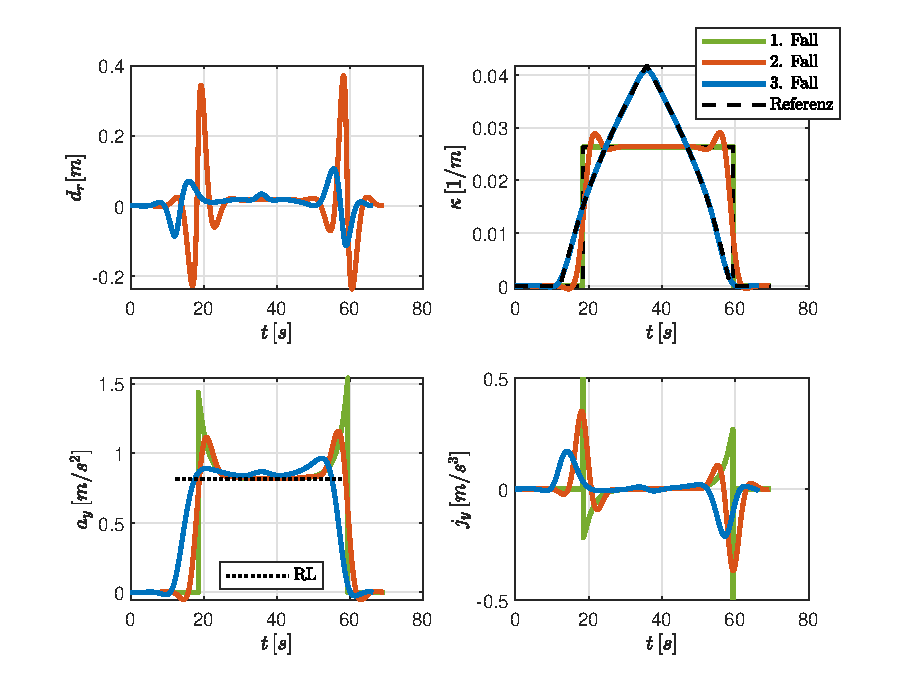
\includegraphics[width=\linewidth]{./Bilder/Ergebnisse/Gerade_Kurve_Gerade/lat_dyn.eps}
	\caption{Trajektorien der Längsdynamik für die drei unterschiedlichen Möglichkeiten zur Beschreibung des Szenarios.}
	\label{fig:gerade_kurve_gerade_lat_dyn}
\end{figure}  
Abgesehen vom veränderten Verlauf der Referenzkrümmung zeigen die Graphen oben links und oben rechts in Abbildung \ref{fig:gerade_kurve_gerade_lat_dyn} noch einen weiteren Unterschied zwischen den Fällen 2 und 3. Die seitliche Abweichung bei Verwendung der Klothoide ist deutlich geringer als in Fall 2 und auch die Abweichung zwischen der optimalen Krümmung und der Referenzkrümmung ist deutlich geringer als in Fall 2. Dies lässt sich damit begründen, dass die Ruckoptimalität, die in Fall 2 auf Kosten der Querabweichung erreicht wird, in der Klothoide bereits in der Referenzkurve berücksichtigt ist. Dadurch kann die optimale Trajektorie deutlich näher an der Referenzkurve selbst gefahren werden. Wie bereits in den vorherigen Abschnitten erläutert wurde, hängt die optimale Querbeschleunigung der (punktweisen) Ruhelage einer Kreis- bzw. Klothoidenfahrt ausschließlich von der Gewichtung der Querbeschleunigung ab. Dadurch ist auch in diesem Szenario gut zu erkennen, dass die Querbeschleunigung in allen drei betrachteten Fällen in der Mitte der Kurvenfahrt gegen \ayRL~verläuft. Der \glqq Hügel\grqq, der in Fall 3 auftaucht, ist darauf zurückzuführen, dass sich das Fahrzeug aufgrund der Krümmungsrampe in der Kurvenmitte kurzzeitig wieder von der punktweisen Ruhelage entfernt. Im Graph unten rechts in Abbildung \ref{fig:gerade_kurve_gerade_lat_dyn} sind schließlich die Verläufe des Querrucks gezeigt, wobei der Querruck im 1. Fall durch numerische Differentiation der Querbeschleunigung und in den Fällen 2 und 3 gemäß Gleichung \eqref{eq:jy} bestimmt wird. Die Ableitung des Sprungs in der Querbeschleunigung führt dabei theoretisch zu unendlich hohen Ruckwerten im 1. Fall. Vergleicht man Fall 2 und Fall 3 miteinander, so ist der Vorteil der Klothoide gegenüber der kreisförmigen Kurvenfahrt hinsichtlich des Querrucks deutlich zu erkennen, da dieser aufgrund der Beschaffenheit der Referenzkurve deutlich stärker reduziert werden kann, als bei der sprunghaften Änderung der Referenzkrümmung. In allen Fällen wird beim Kurvenaustritt der in Abschnitt \ref{subsubsec:Linearisierung} beschriebene Einfluss der instabilen Eigenmoden sichtbar, der dazu verwendet wird, das Fahrzeug aus der Ruhelage zurück in die Geradeausfahrt zu bringen.

\begin{figure}[h] 
	\centering
	\includegraphics[width=\linewidth]{./Bilder/Ergebnisse/Gerade_Kurve_Gerade/svaj.eps}
	\caption{Trajektorien der Längsdynamik für die drei unterschiedlichen Möglichkeiten zur Beschreibung des Szenarios.}
	\label{fig:gerade_kurve_gerade_svaj}
\end{figure}  
Beim Blick auf die Größen der Längsdynamik, welche in Abbildung \ref{fig:gerade_kurve_gerade_svaj} gezeigt sind, fällt ein weiterer Vorteil der Kurve unter Verwendung einer Klothoide auf. Das Fahrzeug ist im 3. Fall um \valunit{2{,}82}{s} schneller, als im 2. Fall und um \valunit{3{,}27}{s} schneller, als im 1. Fall, obwohl die Gesamtstrecke in allen Szenarien identisch ist und die reine Kurvenstrecke, also die Strecke von Kurveneintritt bis Kurvenaustritt bei der Klothoide länger ist, als bei der Kreisfahrt. Für die Fälle 1 und 2 gilt gemäß Gleichung \eqref{eq:Kurvenstrecke} unter Verwendung der konstanten Referenzkrümmung $\kapparef = \valunit{0{,}0263}{\frac{\unit{1}}{\unit{m}}}$, dass die Kurvenstrecke 
\begin{equation}
	s_\textrm{Kurve} = s_2 - s_1 = \frac{2\pi}{\kappa_{\textrm{ref}}} = \valunit{238{,}5022}{m}
\end{equation}
beträgt. Für die Klothoide hingegen lässt sich die Kurvenstrecke durch zwei Halbkreise beschreiben und beträgt daher mit $A = 60$ gemäß Gleichung \eqref{eq:Kurvenstrecke}
\begin{equation}
s_\textrm{Kurve} = 2(s_2 - s_1) = 2\sqrt{\frac{2\pi}{\dkapparef}} = 2\sqrt{2\pi A^2} = \valunit{300{,}7954}{m}\,.
\end{equation}
Der beschriebene Zeitgewinn wird im Graph oben links in Abbildung \ref{fig:gerade_kurve_gerade_svaj} erkennbar und kann damit begründet werden, dass das Fahrzeug beim Durchfahren der Klothoide gegen Ende der Kurve bereits eine deutlich höhere Geschwindigkeit erreicht, wie im Graph oben rechts gezeigt ist. Der Verlauf der Geschwindigkeitstrajektorie von Fall 3 verdeutlicht dabei, dass die optimale Trajektorie in der Kurvendurchfahrt auch in diesem Szenario gegen die punktweise Ruhelage konvergiert. Die Geschwindigkeit der punktweisen Ruhelage der Klothoide ist jedoch krümmungsabhängig, wie in Abschnitt \ref{sec:Klothoide} gezeigt wurde, weshalb diese am Kurvenausgang aufgrund der abnehmenden Referenzkrümmung steigt. Es ist zwar auch zu erkennen, dass die optimale Kurvengeschwindigkeit in den Fällen 1 und 2 in der Kurve ebenfalls gegen die Ruhelage der Kreisfahrt konvergiert, allerdings ist diese aufgrund der konstanten Referenzkrümmung ebenfalls konstant und daher in jedem Punkt der Kurve identisch. Daher verbleibt die optimale Geschwindigkeit in den Fällen 1 und 2 längere Zeit auf dem niedrigeren Geschwindigkeitsniveau. Die unteren beiden Graphen in Abbildung \ref{fig:gerade_kurve_gerade_svaj} zeigen, dass das längsdynamische Verhalten in allen drei Fällen bis zum Kurveneintritt (nach \valunit{18{,}46}{s} bei Fall 1, nach \valunit{18{,}34}{s} bei Fall 2 und nach \valunit{12{,}28}{s} bei Fall 3) identisch ist und die Trajektorien der Längsbeschleunigung und des -rucks qualitativ die aus Abschnitt \ref{sec:Geradeausfahrt} bekannten Verläufe annehmen. Dabei lässt sich feststellen, dass auch die komfortrelevanten Größen in Längsrichtung positiv durch die Klothoide beeinflusst werden. Während die Geschwindigkeit in der Kreisfahrt gegen einen konstanten Wert konvergiert, der lange beibehalten wird und erst am Kurvenausgang unter vergleichsweise starker Änderung der Geschwindigkeit und der Beschleunigung wieder in der Geradeausfahrt mündet, sind die Änderungen der Geschwindigkeit und der Beschleunigung während der gesamten Klothoide zwar stetig, aber dafür vergleichsweise gering. Der Graph unten links zeigt dabei, dass die Beschleunigung innerhalb der Kurve in den Fällen 1 und 2 beinahe Null beträgt. Dieses Abbremsen ist nur unter Verwendung großer Ruckwerte in den Übergangspunkten möglich, wie der Graph unten rechts zeigt. Im Gegensatz dazu unterliegt die Kurvengeschwindigkeit in Fall 3 einer dauerhaften Änderung, was eine stetige Beschleunigung zur Folge hat. Dies wiederum bewirkt in der Kurve einen dauerhaften Längsruck ungleich Null, der jedoch auch an den Übergangspunkten deutlich geringere Werte aufweist und damit einen beträchtlichen Komfortgewinn bewirkt. 

Als Abschluss dieses Kapitels lässt sich festhalten, dass sich die Ergebnisse der zum Teil stark vereinfachten Szenarien auch in der Zusammensetzung von Teilszenarien zu komplexeren Szenarien, wie der Gerade-Kurve-Gerade-Kombination, wiederfinden und daher zur Abschätzung der einzelnen Teilszenarien herangezogen werden können. Zudem konnte gezeigt werden, dass die Beschreibung einer Kurvenfahrt mithilfe einer Klothoide zwar komplizierter ist, aus Sicht des Fahrkomforts jedoch deutlich angenehmere Trajektorien liefert, als eine reine Kreisfahrt und auch hier die Erkenntnisse aus der Analyse der Kreisfahrt weiter verwendet werden können. 